\documentclass[a4paper, 11pt, titlepage, twoside, openany]{book}
\usepackage{plain}
\usepackage{setspace}
% Layout
\usepackage[
  paperheight=29.7cm,
  paperwidth=21cm,
  outer=1.5cm,
  inner=2.5cm,
  top=2cm,
  bottom=2cm
]{geometry}
% Chapter
\usepackage{titlesec}
\singlespacing
\setcounter{secnumdepth}{3}
\setcounter{tocdepth}{3}
% Letter
\usepackage[utf8]{inputenc}
% Language
\usepackage[italian]{babel}
% PDF/A
\usepackage[a-1b]{pdfx}
% Image
\usepackage{graphicx}
\usepackage{wrapfig}
\usepackage{stackengine}
\usepackage{etoolbox}
\BeforeBeginEnvironment{wrapfigure}{\setlength{\intextsep}{0pt}}
% Hyperlink
\usepackage{xurl}
\usepackage[pdfa]{hyperref}
\hypersetup{
  breaklinks=true,
  colorlinks=true, % Colora i link invece di usare riquadri colorati
  linkcolor=black, % Colore dei link interni (indice, sezioni)
  citecolor=black, % Colore delle citazioni
  filecolor=black, % Colore dei link ai file locali
  urlcolor=black % Colore degli URL
}
\usepackage{nameref}
% List
\usepackage{enumitem}
\usepackage{array}
% Symbols
\usepackage{pifont}
\newcommand{\cmark}{\textcolor{green}{\ding{51}}}
\newcommand{\xmark}{\textcolor{red}{\ding{55}}}
\newcommand{\imark}{\textcolor{orange}{\ding{118}}}
% Code
\usepackage{listings}
\usepackage{xcolor}
\definecolor{codeaqua}{RGB}{104,157,106}
\definecolor{codegray}{RGB}{124,111,100}
\definecolor{codepurple}{RGB}{177,98,134}
\definecolor{codered}{RGB}{204,36,29}
\definecolor{backcolour}{RGB}{249,245,215}
\lstdefinestyle{mystyle}{ backgroundcolor=
\color{backcolour}
, commentstyle=
\color{codepurple}
, keywordstyle=
\color{codered}
, numberstyle=\tiny
\color{codegray}
, stringstyle=
\color{codeaqua}
, basicstyle=\ttfamily\footnotesize, breakatwhitespace=false, breaklines=true, captionpos=b,
keepspaces=true, numbers=left, numbersep=5pt, showspaces=false, showstringspaces=false,
showtabs=false, tabsize=2, }
\lstset{style=mystyle}
% Configure siunitx for Italian number formatting
\usepackage{siunitx}
\sisetup{ output-decimal-marker = {,}, group-separator = {.}, group-minimum-digits = 4 }

% Document
\begin{document}
  % Cover
  \pagenumbering{gobble}
  \pagestyle{plain}
\thispagestyle{empty}

\begin{center}
  \begin{figure}[h!]
    \centering
    
\includegraphics[width=.6\textwidth]{images/logo/unitn.eps}
  \end{figure}

  \vspace{2 cm}
  \LARGE{Dipartimento di Ingegneria e Scienza dell'Informazione\\}

  \vspace{1 cm}
  \Large{Laurea Triennale in\\ Informatica}

  \vspace{2 cm}
  \Large\textsc{Elaborato Finale\\}
  \vspace{1 cm}
  \Huge\textsc{Modernizzazione della piattaforma di Cyber Threat Intelligence
  SATAYO\\}
  \vspace{0.5 em}
  \Large{\textit{L'impatto del debito tecnico sulla scalabilità delle applicazioni}}

  \vspace{2 cm}
  \begin{tabular*}{\textwidth}{c @{\extracolsep{\fill}} c}
    \Large{Supervisore}             & \Large{Laureando}          \\
    \Large{Prof. Bruno Crispo}      & \Large{Lorenzo Bevilacqua} \\
    \Large{Co-Supervisore}          & \Large{226730}             \\
    \Large{Dr. Francesco Pavanello} & {}                         \\
  \end{tabular*}

  \vspace{2 cm}
  \Large{Anno Accademico 2023/2024}
\end{center}
  \clearpage

  % Acknowledgements
  \thispagestyle{empty}

\begin{center}
  {\bf \Huge Ringraziamenti}
\end{center}

\vspace{4cm}
\emph{Thanks to ...}
  \clearpage
  \pagestyle{plain}

  % Table of Contents
  \frontmatter
  \pagenumbering{Roman}
  \tableofcontents
  \clearpage
  \begingroup
  \pagestyle{empty}
  \cleardoublepage
  \endgroup

  % Start page numbering
  \mainmatter

  % Group to define space between chapters
  \begingroup
  % Override format of title chapter
  \titleformat{\chapter} {\normalfont\Huge\bfseries}{\thechapter}{1em}{} \titlespacing*{\chapter}{0pt}{0.59in}{0.02in}
  \titlespacing*{\section}{0pt}{0.20in}{0.02in} \titlespacing*{\subsection}{0pt}{0.10in}{0.02in}
  \titlespacing*{\subsubsection}{0pt}{0.05in}{0.02in}

  % Abstract
  \chapter*{Abstract}
\label{cha:abtract}
\addcontentsline{toc}{chapter}{Abstract}

SATAYO è una piattaforma di Cyber Threat Intelligence, completamente sviluppata da
Würth Phoenix, che permette di monitorare l'esposizione online di un'organizzazione
e di individuare anticipatamente eventuali minacce cyber. In questo elaborato verrà
trattata l'architettura iniziale del progetto e le problematiche presenti che ne
impedivano la scalabilità. Verranno individuati e analizzati i requisiti da
soddisfare durante il processo di modernizzazione, e descritto il processo utilizzato
per individuare la soluzione più adatta al problema presentatosi. Verrà infine
introdotto Apache Airflow, progetto Open source, che prenderà il posto del core
dell'implementazione attuale permettendo una maggiore scalabilità e migliore
gestione delle fasi di ricerca.

  % Chapters
  \chapter{Introduzione}
\label{cha:introduction}

% discorso unico generico in cui parli dell'azienda, del SOC e di cosa ti è stato richiesto
  \chapter{Background}
\label{cha:background}

In questo capitolo verrà descritta la piattaforma oggetto di studio, saranno inoltre
introdotte delle definizioni e concetti generali riguardanti la Threat Intelligence
e la Open Source Intelligence.

\section{SATAYO}
\label{sec:satayo}

Come accennato precedentemente, SATAYO\cite{satayo} è un servizio che colleziona,
aggrega e presenta informazioni di natura OSINT in modo semi automatico. È
disponibile in modalità \textit{One Time}, in cui un cliente può richiedere uno
scan della propria esposizione, il quale sarà consultabile per qualche settimana;
\textit{SaaS (Software as a Service)}, in cui viene continuamente monitorata l'esposizione
online di un cliente con la possibilità di consultare direttamente la
piattaforma; infine in modalità \textit{SaaS \& Managed} in cui, oltre all'accesso
diretto come in modalità SaaS, il cliente ha anche a disposizione un team di
specialisti che analizzano le evidenze collezionate e forniscono direttamente
istruzioni per eventuali mitigazioni necessarie. Le ricerche di SATAYO sono quasi
completamente automatizzate, vengono infatti svolte le azioni necessarie per il
collezionamento delle risorse senza intervento manuale: per esempio partendo da un
dominio, automaticamente vengono trovati i suoi sotto domini, che a loro volta verranno
analizzati per testare eventuali servizi esposti. Contrariamente azioni come l'inserimento
di metadati del cliente per perfezionare le ricerche, e il controllo qualità a fine
ricerca, previa pubblicazione, vengono svolte manualmente da un analista. SATAYO
non è limitato alle risorse presenti nel \textit{Surface Web}\cite{Kavallieros2021},
esegue infatti ricerche e utilizza informazioni presenti nel \textit{Deep Web}, ovvero
la parte di internet non indicizzata dai motori di ricerca, e nel \textit{Dark
Web} che è accessibile solo tramite software specifici come \texttt{Tor}\footnote{\url{https://www.torproject.org/}}.
In questa ultima porzione di internet è possibile trovare anche piattaforme in
cui vengono venduti oggetti e software illegali, come può essere l'accesso privilegiato
all'infrastruttura di un cliente.

\section{OSINT}
\label{sec:osint}

L'OSINT\cite{GLASSMAN2012673}, ovvero Open Source INTelligence, è una branca dell'intelligence
che si occupa della ricerca e analisi di dati ottenuti da fonti accessibili pubblicamente.
In generale queste informazioni possono essere ottenute da risorse di diverso
tipo, quali mezzi di comunicazione (giornali, riviste, televisione), dati
governativi pubblici, pubblicazioni accademiche, dati commerciali e, soprattutto,
dall'internet. È proprio quest'ultima la fonte principale utilizzata da SATAYO,
online infatti si trovano molte informazioni che per natura devono essere
pubbliche, ma spesso non ci si presta attenzione. Esempi di queste informazioni
possono essere: record DNS, i quali rivelano molte informazioni riguardanti il
perimetro pubblico di un'organizzazione; account su piattaforme di social network,
quali Linkedin, che riportano in modo piuttosto dettagliato la lista di dipendenti
di un'azienda con i rispettivi ruoli all'interno della stessa; market nel
\textit{Dark Web} che mettono in vendita informazioni che possono essere ritenute
pericolose se di dominio pubblico, come log rubati da macchine infette e accesso
privilegiato alla rete aziendale.

\begin{figure}[htbp]
  \centering
  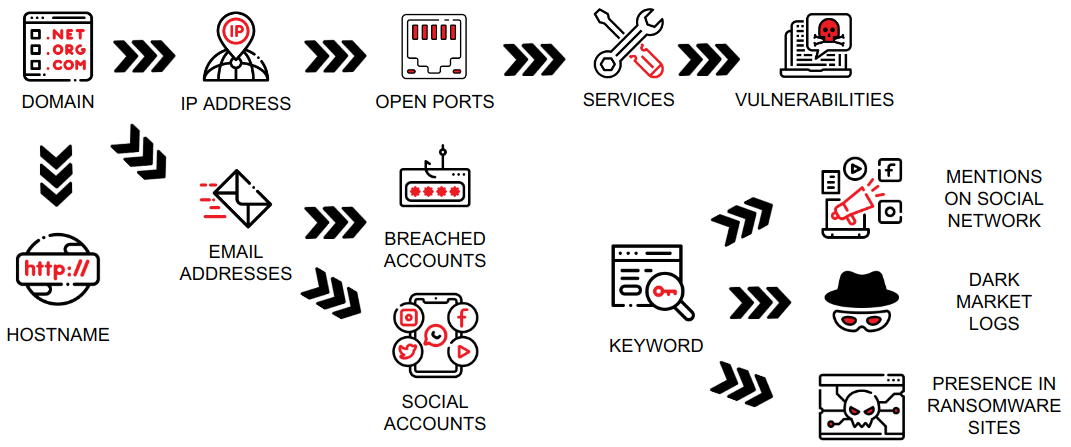
\includegraphics[width=.7\linewidth]{images/exposure_assessment.png}
  \caption{Esempio di informazioni collezionate con metodologie OSINT\cite{pavanello-master}}
  \label{fig:exposure_assessment}
\end{figure}

\pagebreak
\section{Cyber Threat Intelligence}
\label{sec:cti}

La \textit{Cyber Threat Intelligence}\cite{lee2023cyber} (CTI) rappresenta l'analisi
di intelligence ottenuta tramite fonti OSINT, file di log, analisi del traffico
di rete di un'organizzazione e analisi forensi. Lo scopo della CTI è di studiare
e individuare delle possibili minacce, sia cyber che fisiche, in modo tale da agire
proattivamente agli attacchi che si potrebbero presentare in futuro. Grazie a
questa tecnica per le aziende è possibile individuare quali minacce presentano
un rischio maggiore e agire di conseguenza. Parte della CTI è anche l'individuazione
di \textit{Threat Actors}, persone o gruppi di persone che pongono una minaccia nei
confronti di aziende e organizzazioni. Solitamente si ottengono evidenze di
questi TA tramite ricerche nel deep o dark web, vengono poi correlate le informazioni
ottenute con altri dati riguardanti i clienti per individuare eventuali minacce.
  \chapter{Architettura iniziale}
\label{cha:architettura_iniziale}

In questo capitolo viene descritto lo stato iniziale di SATAYO, la sua complessità
e i problemi di scalabilità che hanno portato alla necessità di ripensare l'architettura
del progetto.

\section{Struttura del progetto}
\label{sec:struttura}

Il progetto SATAYO è strutturato in modo tale da permettere la distribuzione del
lavoro su più macchine virtuali. In questo modo, dal punto di vista teorico, dovrebbe
essere più semplice scalare l'applicazione in base alla quantità e alla dimensione
dei domini che vengono analizzati dalla piattaforma.

\begin{figure}[h!]
  \centering
  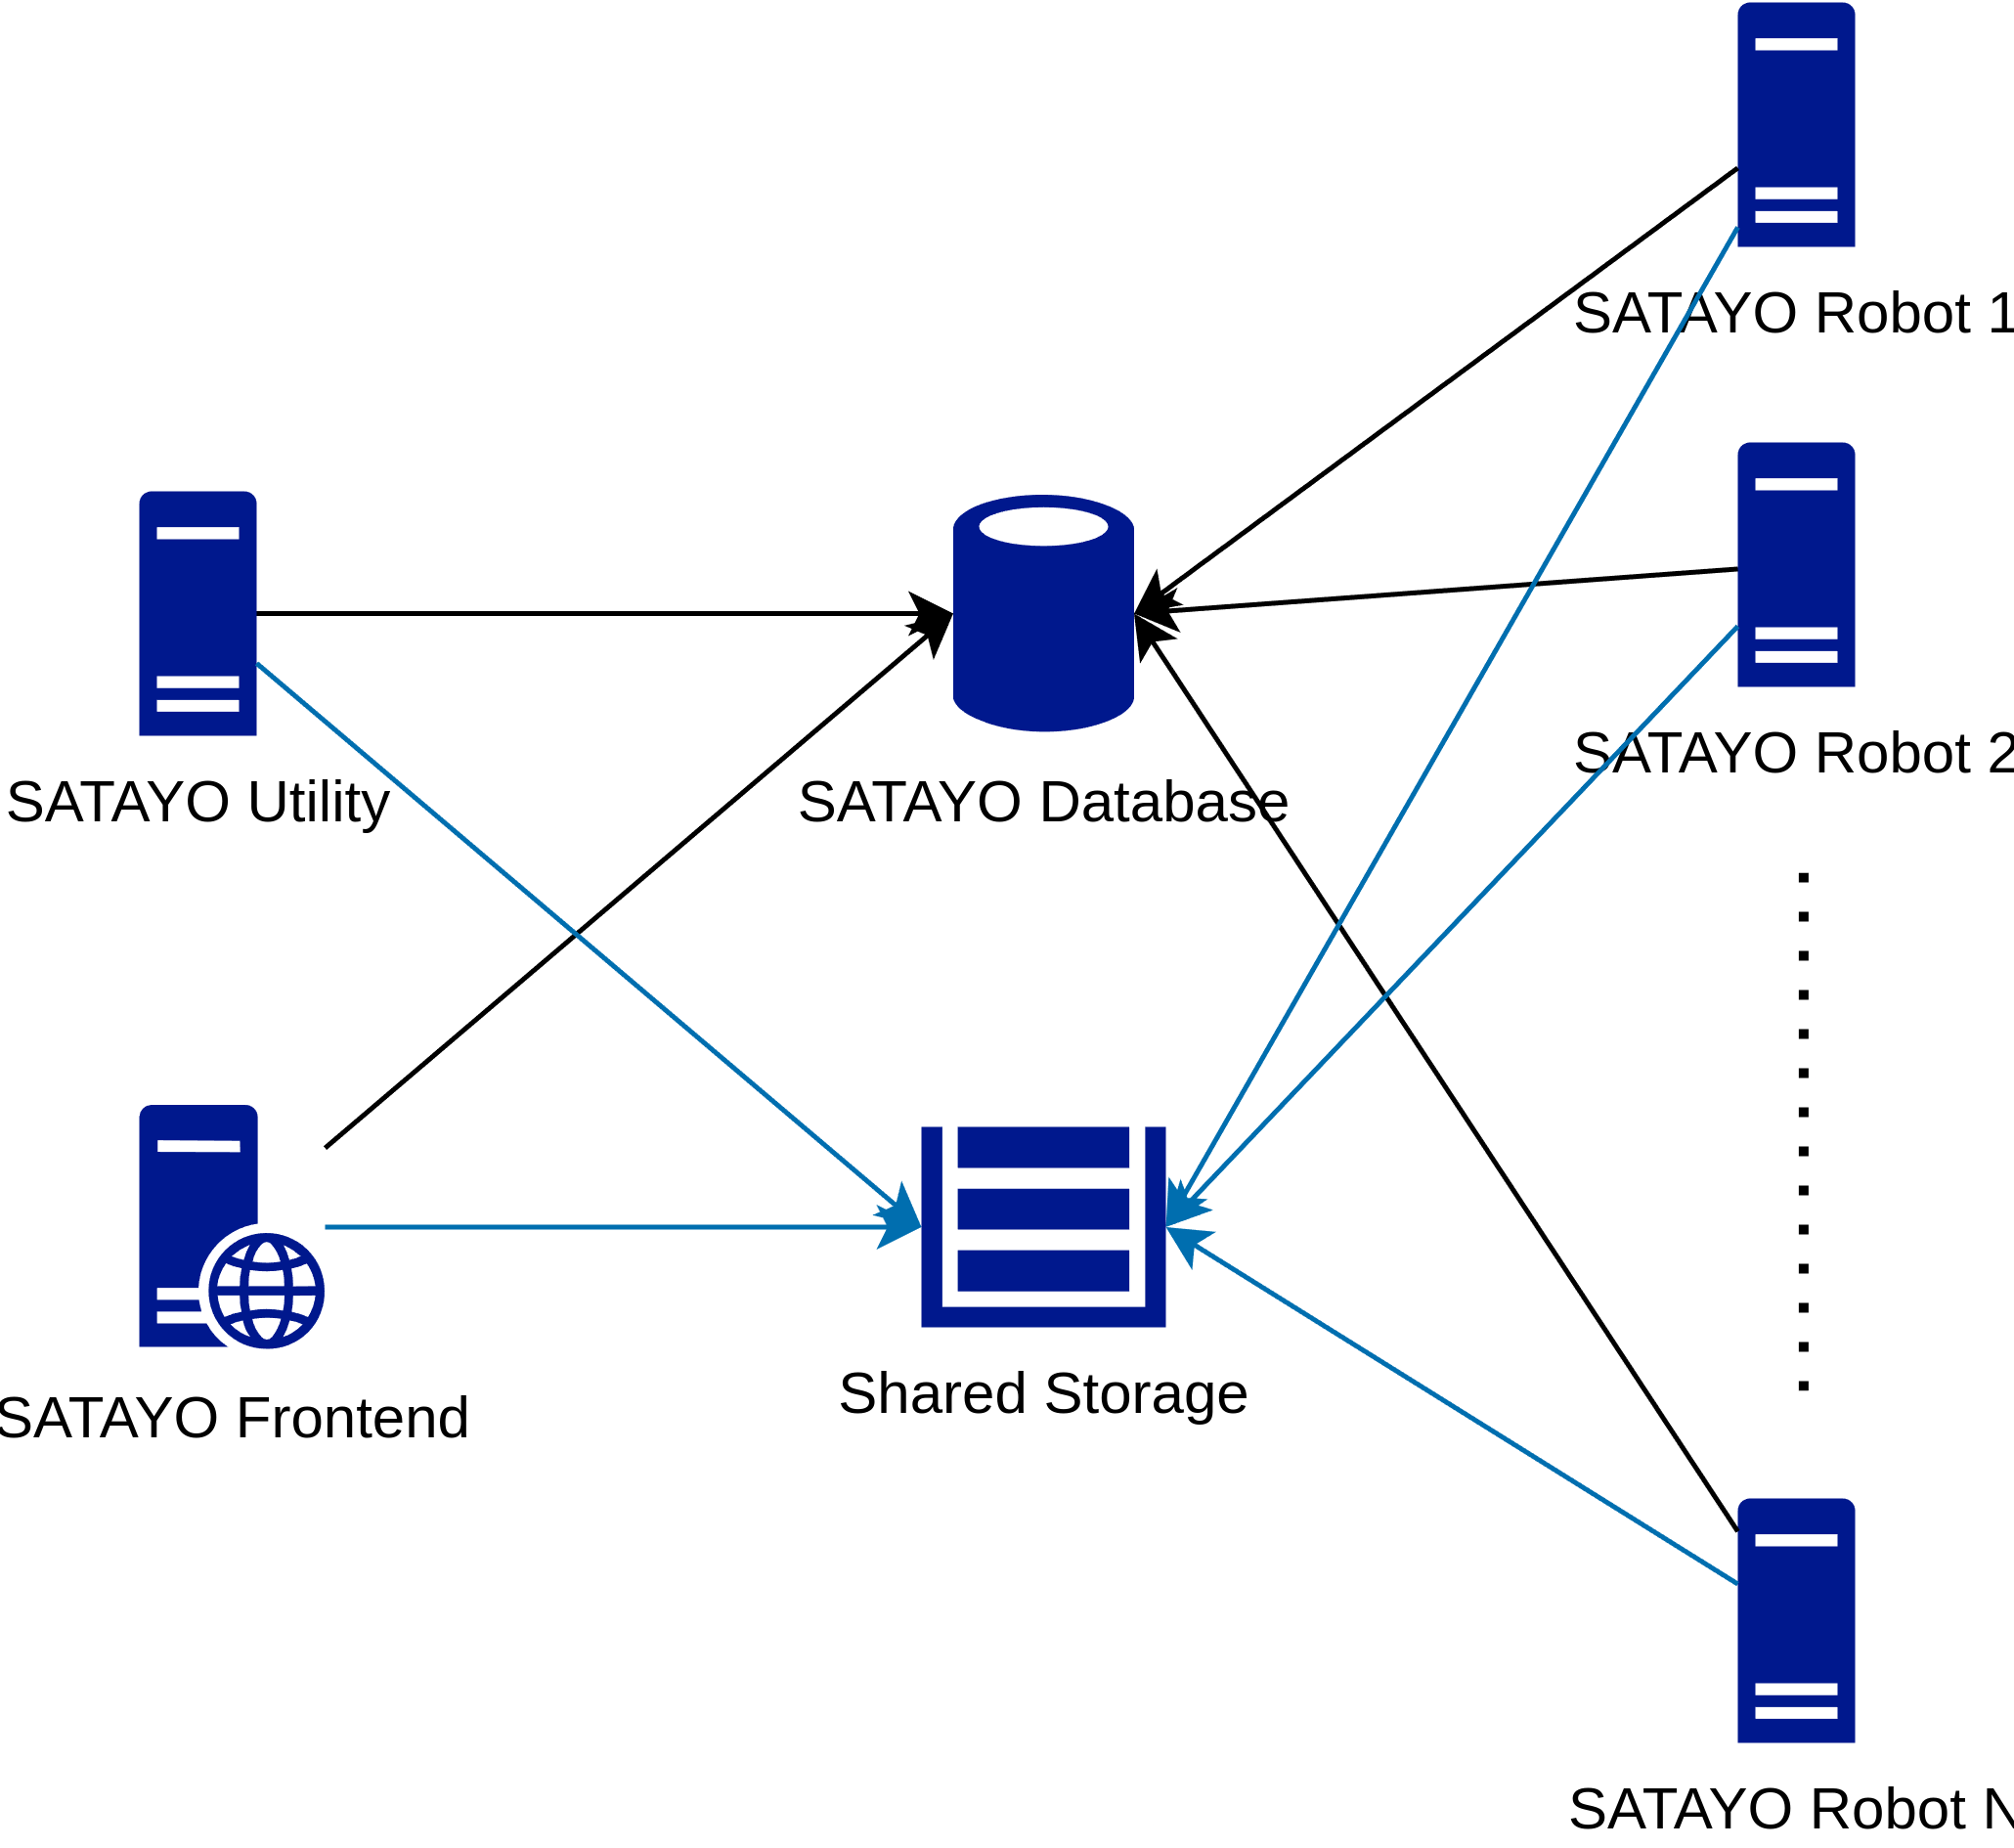
\includegraphics[width=.6\linewidth]{images/SATAYO_infrastructure_old.png}
  \caption{Vecchia infrastruttura di SATAYO}
  \label{fig:infra_old}
\end{figure}

Come si nota in figura \ref{fig:infra_old}, sono presenti tre categorie di macchine
con compiti distinti:

\begin{itemize}
  \item \textbf{SATAYO Frontend:} dedicata all'hosting del webserver con cui
    clienti e analisti si interfacciano per utilizzare la piattaforma. Questa macchina
    ha la necessità di interfacciarsi con il database, per leggere i dati
    generati da SATAYO e per inserire nuovi domini o informazioni relative a
    questi nella piattaforma. La stessa macchina ha inoltre bisogno di permessi di
    lettura sullo storage condiviso, in cui vengono salvate le evidenze trovate
    sulle varie piattaforme OSINT da SATAYO, per presentarle agli analisti che ne
    devono valutare la correttezza e gravità;

  \item \textbf{SATAYO Utility:} la sua funzione principale è quella di eseguire
    fasi molto scalabili orizzontalmente; fasi cioè, il cui tempo di esecuzione
    e carico sul sistema non dipende affatto o dipende in minima parte dal
    numero di input. Esempi specifici di queste esecuzioni possono essere lo scraping
    di siti web o di canali Telegram. Come la SATAYO Frontend anche SATAYO
    Utility comunica con il database, principalmente per inserire dati, e con lo
    storage condiviso per salvare evidenze collezionate da fonti varie;

  \item \textbf{SATAYO Robot:} argomento principale di questo elaborato, ha il compito
    di eseguire tutte le fasi legate ad un particolare dominio. Generalmente si
    tratta di programmi e tool open-source o di terze parti che lavorano su
    input singoli, non permettendo così una parallelizzazione analoga alle fasi Utility.
    Altra particolare caratteristica delle macchine Robot, che verrà analizzata più
    nel dettaglio al punto \ref{sub:robots}, è la necessità di eseguire le
    operazioni secondo un insieme di dipendenze. Per esempio, una funzione che
    ritorna una lista di servizi online a cui sono iscritti i dipendenti tramite
    email aziendali, deve essere eseguita dopo la fase che si occupa di raccogliere
    la lista di dipendenti di una determinata azienda. Questa famiglia di
    macchine, come la SATAYO Utility, si interfaccia direttamente con il
    database e con lo storage condiviso.
\end{itemize}

In fine è presente il database, il quale è ospitato su una macchina dedicata per
poter garantire una performance migliore. Quest'ultima, analogamente allo storage
condiviso, è protetta da policy di sicurezza più strette rispetto alle altre
macchine che hanno bisogno di comunicare e interagire con la rete esterna.

\subsection{Macchine Robot}
\label{sub:robots}

Di seguito verranno trattati più approfonditamente l'architettura, il
funzionamento e il controllo delle macchine Robot.

Come visto in precedenza queste macchine eseguono operazioni secondo un grafo di
dipendenze, le quali sono definite in modo implicito nei metadati delle singole fasi.
Con il termine \textit{dipendenze implicite} si intende che non è presente una rappresentazione
in cui si può osservare chiaramente l'ordine con cui devono essere eseguite le fasi,
ma bensì sono presenti delle impostazioni che definiscono, per ogni funzione, la
famiglia di fasi che si devono essere concluse prima che possa essere eseguita
quest'ultima.

L'esecuzione delle fasi viene gestita in modo piuttosto rudimentale: su ogni istanza
Robot è presente uno script Python \texttt{satayo.py} il quale viene eseguito da
un Crontab secondo un intervallo regolare di 5 minuti. Questo script è a tutti gli
effetti il controllore locale della macchina Robot, ha il compito di eseguire le
fasi presenti nella coda di quell'istanza e di controllare lo stato di
esecuzione di esse. Più nel dettaglio lo script esegue le seguenti operazioni:

\begin{itemize}
  \item controlla se l'esecuzione avviata con il cronjob precedente è ancora attiva,
    in tale caso non viene avviata nessuna nuova fase. In caso l'esecuzione precedente
    sia terminata si controlla che non ci siano stati errori nell'esecuzione, in
    caso positivo viene salvato sul database l'errore e gli eventuali messaggi
    di log.

  \item è selezionata la prossima fase da eseguire tramite lookup sulla tabella di
    coda nel database. Si eseguono dei controlli per verificare che le
    dipendenze di quest'ultima siano soddisfatte. Infine si avvia l'esecuzione effettiva
    della task.

  \item una volta terminata l'esecuzione vengono salvati i risultati dell'operazione,
    gli eventuali messaggi di log, lo stato finale dell'esecuzione, e la
    macchina rimane in attesa del prossimo cronjob.
\end{itemize}

Si possono immediatamente notare delle forti inefficienze, le quali saranno trattate
dettagliatamente al punto \ref{sec:problemi}:

\begin{itemize}
  \item l'intervallo del Crontab è stato calcolato in modo arbitrario secondo una
    stima della media pesata dei tempi di esecuzione delle varie fasi. Ciò
    significa che alcune esecuzioni sono molto più rapide rispetto all'intervallo
    e viene quindi sprecato tempo macchina;

  \item su ogni istanza può essere eseguita soltanto una fase alla volta, non è
    supportata l'esecuzione parallela sulla stessa macchina. La scelta fatta per
    cercare di mitigare questo problema è stata duplicare l'istanza su più macchine
    indipendenti e implementare la logica per gestire la distribuzione della coda.
\end{itemize}

L'approccio descritto è il risultato di un'aggiunta incrementale di funzionalità,
effettuata mantenendo la semplice struttura iniziale, ormai inadatta al carico
di lavoro e alla complessità del progetto.

La coda di esecuzione e i metadati delle fasi verranno trattati al punto
\ref{sec:database} assieme ad altri dettagli relativi al database.

\section{Struttura database}
\label{sec:database}

Il database di SATAYO, inizialmente formato da circa 50 tabelle, ne conta ad oggi
oltre 130. Non essendo possibile citare e descriverle tutte, vengono riportate
quelle principali e più inerenti ai problemi e alle modifiche che verranno
descritte al capitolo \ref{cha:nuova_architettura}.

\textbf{\textit{INSERIRE ER TABELLE (2 cluster): ui\_org, domain, research | tool\_progress,
tool, host, log}}

\subsection{Gestione clienti, domini e ricerche}
\label{sub:db:mgmt}

Il primo cluster di tabelle, rappresentato sulla sinistra in figura \textbf{\textit{X}}
forma il cuore del database di SATAYO, queste sono infatti tabelle che
contengono i dati del cliente, dei domini da analizzare e delle ricerche OSINT effettuate
sui vari domini. Nel dettaglio le tabelle rappresentate contengono le seguenti
informazioni:

\begin{itemize}
  \item \textbf{ui\_org:} contiene le informazioni relative ai clienti, quali:
    date di inizio e fine del contratto, collegamenti a software ERP interno,
    tipologia di contratto e funzionalità abilitate e altre informazioni di
    natura burocratica. Nel contesto tecnico svolge la funzione di permettere una
    gestione d'insieme dei domini e delle ricerche di un determinato cliente;

  \item \textbf{domain:} racchiude i domini monitorati per un determinato
    cliente. Oltre al dominio stesso contiene anche altre informazioni di contesto
    quali: keyword per eseguire ricerche online, nomi degli account di piattaforme
    di social media per verificare le informazioni esposte pubblicamente e formato
    delle mail aziendali per enumerare i dipendenti.

  \item \textbf{research:} in fase di progettazione iniziale, è stato individuato
    come requisito la possibilità di offrire uno storico della propria esposizione
    in rete al cliente. Ciò ha portato alla necessità di implementare questa
    tabella che ha il compito di rendere discrete le ricerche che vengono
    effettuate, permettendo quindi una visualizzazione distinta nel tempo dell'andamento
    delle evidenze ed esportabile in un report.
\end{itemize}

\subsection{Gestione fasi}
\label{sub:db:tasks}

Il secondo cluster, presente sulla destra della figura \textbf{\textit{X}}
contiene invece informazioni di natura operativa, quali code di esecuzione e metadati
delle fasi. Le funzionalità principali sono le seguenti:

\begin{itemize}
  \item \textbf{tool:} è una lista statica dei tool OSINT implementati su SATAYO,
    che ad oggi sono oltre 60. Contiene il nome dei singoli tool, l'ordine in
    cui devono essere eseguiti, assieme a metadati usati per la distribuzione su
    più host e per la gestione da frontend;

  \item \textbf{host:} un'altra lista statica contenente tutti gli hostname, e altre
    informazioni di gestione, delle macchine che formano la piattaforma SATAYO, come
    visto in figura \ref{fig:infra_old}. Al momento sono presenti 12 macchine
    Robot. Le informazioni contenute in questa tabella hanno la funzione principale
    di gestire la distribuzione delle fasi tra le diverse macchine Robot;

  \item \textbf{tool\_progress:} contiene lo stato di esecuzione delle singole
    fasi. Più nel dettaglio contiene informazioni quali: lo stato, cioè se una task
    può essere eseguita, è in esecuzione o è terminata con errore o con successo,
    e l'orario di inizio e di fine dell'esecuzione. Inoltre contiene anche le
    seguenti informazioni: tool da eseguire, host su cui viene eseguito e
    ricerca su cui caricare le evidenze collezionate dal tool;

  \item \textbf{log:} semplice tabella utilizzata per salvare messaggi di log
    provenienti dalle esecuzioni dei vari tool. Contiene il tempo di creazione del
    log, la gravità e il messaggio di log stesso. È utile per individuare problemi
    durante le esecuzioni di task direttamente dal frontend.
\end{itemize}

\pagebreak
\section{Problemi con architettura corrente}
\label{sec:problemi}

In seguito ad un'analisi di carico e ad una proiezione del numero di domini da
monitorare nei prossimi mesi, sono risultati immediatamente evidenti i problemi di
scalabilità che si sarebbero presentati se si fosse mantenuta l'architettura attuale.

Come accennato nelle sezioni precedenti, l'implementazione corrente permette di
scalare orizzontalmente in modo teoricamente semplice: se c'è bisogno di ulteriore
tempo di esecuzione è sufficiente aggiungere un'altra macchina Robot,
configurarla secondo una data documentazione e aggiungere eventuali entry nel
database. Questa può essere una valida soluzione in caso non sia necessario eseguire
la procedura molto spesso. Contrariamente, se fosse necessario scalare in modo più
che lineare, questa soluzione porterebbe ad un \textbf{notevole dispendio di
tempo} per la configurazione iniziale, ma soprattutto per la gestione e
manutenzione futura del sistema.

Un altro problema, a cui porterebbe un simile approccio, è lo \textbf{spreco di
risorse}: dal momento che l'implementazione attuale non può sfruttare al meglio
multipli core, per utilizzare in modo efficiente le risorse messe a disposizione
dall'infrastruttura sottostante, è necessario creare macchine con requisiti
minimi. Prendendo come riferimento la guida di Ubuntu Server\footnote{\url{https://ubuntu.com/server/docs/system-requirements}},
sistema operativo utilizzato su tutte le istanze, e aumentando lievemente le
risorse minime per poter eseguire anche le fasi più computazionalmente intensive,
si ottengono dei requisiti di 2 CPU core, 8GB di RAM e 60GB di spazio di
archiviazione. Questo porta il totale di risorse in utilizzo, considerando solo
le macchine Robot, a 24 CPU core, 96GB di RAM e 720GB di spazio di archiviazione,
la maggior parte delle quali non è possibile sfruttare appieno.

Terza criticità è la gestione dei log, i quali al momento vengono collezionati
tramite query direttamente sul database di SATAYO. Questo può portare ad alcune situazioni
in cui certi errori non vengono riportati correttamente; un esempio può essere
il caso in cui si perda la connessione con il database, la fase andrebbe in errore
ma non verrebbe correttamente riportato il messaggio di log.
  \chapter{Analisi prerequisiti e possibili soluzioni}
\label{sec:analisi_ricerca}

Una volta esaminata l'implementazione attuale e identificati i suoi principali
problemi nel capitolo precedente, è stato deciso di utilizzare un approccio DRY.
L'acronimo DRY, Don't Repeat Yourself, si riferisce al principio in Computer
Science in cui "Ogni conoscenza deve avere una rappresentazione unica, univoca e
autorevole all’interno di un sistema" descritto in \texttt{The Pragmatic
Programmer}\cite{thomas2019pragmatic}. In questo caso ne viene esteso il
significato per riferirsi all'utilizzo di framework esterni testati e che hanno
dimostrato di funzionare.

\section{Prerequisiti}
\label{sec:prerequisiti}

Viene proposta ora un'analisi esaustiva dei prerequisiti da considerare e valutare
durante il processo di ricerca \ref{sec:candidates} e scelta \ref{sec:airflow} del
framework che verrà usato per sostituire l'attuale implementazione. Si
individuano i prerequisiti fondamentali riportati di seguito.

\subsection{Utilizzo efficiente delle risorse}
\label{sub:resource_usage}

Primo prerequisito fondamentale è la possibilità di sfruttare completamente le risorse
a disposizione. Questo significa che bisognerà inizialmente favorire la
scalabilità verticale del sistema, in questo modo è possibile partire da un sistema
più semplice che verrà esteso in seguito. Scalare verticalmente comporta creare
una macchina unica più potente e risparmiare nel complesso risorse, in quanto l'overhead
del sistema operativo è presente soltanto una volta e un core può effettivamente
eseguire più task alla volta sfruttando il multithreading.

\subsection{Definizione dipendenze tramite DAG}
\label{sub:deps_definition}

Come visto nella sezione \ref{sub:robots}, vengono definite delle dipendenze tra
fasi. Uno dei prerequisiti fondamentali è la possibilità di definire in modo
esplicito grafi di dipendenze, non dovendo quindi pensare per ogni fase quali devono
essere quelle che la precedono o la seguono. Sarebbe ideale un'implementazione
analoga a quella riportata nel codice \ref{lst:dag-example} e renderizzata in
figura \ref{fig:dag-example}.

\begin{figure}[htbp]
  \centering
  \begin{minipage}{0.45\textwidth}
    \centering
    \lstinputlisting[language=Python, caption=Esempio di definizione di DAG in Airflow,
    label=lst:dag-example ]{listings/dag-example.py}
  \end{minipage}
  \hfill
  \begin{minipage}{0.45\textwidth}
    \centering
    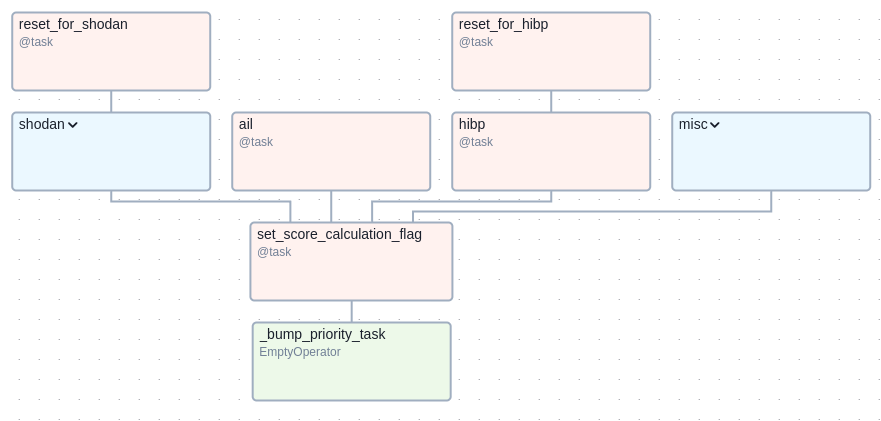
\includegraphics[width=\textwidth]{images/dag-example.png}
    \caption{Esempio di renderizzazione del DAG}
    \label{fig:dag-example}
  \end{minipage}
\end{figure}

\subsection{Compatibilità con Python}
\label{sub:python_compatibility}

Il linguaggio di programmazione principale, in cui è scritta la parte di collezione
e serializzazione dei dati, è Python. Questo significa che gran parte delle fasi
eseguite dalle macchine Robot possono essere utilizzate nella nuova implementazione
senza cambiamenti radicali. Data la natura della maggior parte delle task, che svolgendo
ricerche OSINT, vengono eseguite molte richieste di rete. Ciò significa che, per
la maggior parte del tempo, il processo resta in attesa di una risposta da un server
remoto (I/O intensive) e non esegue operazioni computazionalmente pesanti (CPU
intensive). Per questo motivo utilizzare un linguaggio di programmazione più
performante non aumenterebbe molto le prestazioni e aggiungerebbe soltanto
complessità nel tradurre le implementazioni attuali e gestire codice in un
linguaggio poco conosciuto dal team.

Un'altra caratteristica fondamentale e correlata è la possibilità di definire le
task in modo programmatico, in modo da appunto riutilizzare il codice già presente
e funzionante.

\subsection{Scalabilità orizzontale}
\label{sub:scalable}

Espandendo quanto descritto al requisito \ref{sub:resource_usage}, potrebbe presentarsi
la necessità di scalare e utilizzare più risorse di quelle messe a disposizione dall'infrastruttura
sottostante. Questo problema può essere risolto utilizzando un approccio di
scalabilità orizzontale. Il framework selezionato deve quindi offrire la possibilità
di funzionare su cluster in modo relativamente semplice e veloce, idealmente
utilizzando soluzioni ben conosciute quali Kubernetes\cite{kubernetes}.

\subsection{Open source, Manutenzione e Documentazione}
\label{sub:open_source}

Prima di valutare strumenti offerti da altre aziende come prodotti a pagamento, è
opportuno valutare la presenza di eventuali strumenti Open source o disponibili gratuitamente.
In ambito Open source bisogna prestare particolare attenzione a tre aspetti
chiave: la manutenzione, ovvero quanto attivo è il progetto e quanto velocemente
vengono risolti bug e implementate nuove funzionalità; il supporto, ovvero
quanto è attiva la comunità attorno al progetto per chiedere aiuto in caso di
problemi o difficoltà nell'utilizzo del framework; completezza e chiarezza della
documentazione, fondamentale per utilizzare in modo efficiente tutte le
funzionalità del software in questione.

\subsection{Isolabilità}
\label{sub:isolation}

Alcune fasi implementate all'interno di SATAYO necessitano di un ambiente isolato
per essere eseguito correttamente. Esempio pratico di questo requisito potrebbe
essere l'utilizzo di una VPN, che forza tutto il traffico del sistema ad uscire attraverso
di essa; questo non permetterebbe a determinate altre fasi di comunicare
correttamente con il server remoto a cui si appoggiano. Analogamente se una determinata
fase utilizza un software Open source di dubbia sicurezza, o con dipendenze
molto vecchie che andrebbero in conflitto con il resto del sistema, è opportuno che
vengano eseguite le fasi all'interno di sandbox che ne limitino le capacità.

\subsection{Monitorabilità}
\label{sub:monitorable}

Ultimo requisito fondamentale è la possibilità di poter monitorare a fondo lo
stato del sistema, ma soprattutto lo stato delle singole fasi che sono in esecuzione.
Più specificatamente è necessario avere una visione molto dettagliata della
parte di schedulazione implementata dal framework, il quale deve mettere a disposizione
metriche collezionabili da sistemi di monitoraggio quali Neteye\cite{neteye} o
Prometheus\footnote{\url{https://prometheus.io/}}.

Per quanto riguarda il collezionamento dei log di esecuzione delle fasi, deve
esserci un metodo standardizzato per produrli in modo tale che possano essere
collezionati da sistemi di collezionamento e indicizzazione come Elasticsearch\footnote{\url{https://www.elastic.co/elasticsearch}}.

\section{Soluzioni candidate}
\label{sec:candidates}

Durante l'attività di ricerca sono state individuate più soluzioni e framework
che rispettavano alcuni o tutti i requisiti definiti nella sezione precedente. Di
seguito sono riportate le caratteristiche dei candidati più interessanti che sono
stati valutati per la scelta finale, la tabella \ref{table:requisites} riporta
una visualizzazione di tutti i requisiti per ogni framework.

\begin{itemize}
  \item \textbf{multithreading nativo di Python:} prima possibile soluzione, è stata
    immediatamente scartata in quanto rispetta solo il requisito \ref{sub:resource_usage}
    (e naturalmente \ref{sub:python_compatibility}). Nonostante ciò è risultata
    molto utile per individuare correttamente il requisito \ref{sub:open_source};

  \item \textbf{Celery\footnote{\url{https://docs.celeryq.dev/en/stable/}}:} è
    il primo framework effettivo analizzato come possibile opzione, dalla documentazione
    ufficiale "Celery è un sistema distribuito semplice, flessibile e affidabile
    per elaborare grandi quantità di messaggi, fornendo al tempo stesso alle
    operazioni gli strumenti necessari per mantenere tale sistema". Data questa
    definizione Celery sembra un ottimo candidato, soddisfa pienamente i requisiti:
    \ref{sub:resource_usage} in quanto un nodo worker può sfruttare al meglio le
    risorse eseguendo più fasi in diversi sottoprocessi; \ref{sub:python_compatibility}
    perché scritto interamente in Python e completamente compatibile con esso;
    \ref{sub:open_source} in quanto il progetto è molto grande e mantenuto. Contrariamente
    in Celery non esiste un modo conciso di definire dipendenze tramite DAG,
    \ref{sub:deps_definition}. Esiste la possibilità di scalare orizzontalmente come
    richiesto da \ref{sub:scalable} aggiungendo nodi worker al sistema, bisogna
    però gestirli manualmente e non può essere delegato a piattaforme pre
    esistenti quali Kubernetes. Infine rispetta parzialmente anche il requisito \ref{sub:isolation}
    in quanto nonostante non ci sia un metodo nativo di implementarlo, si
    possono creare più worker in ambienti dedicati diversi, ed eseguire determinate
    task con requisiti particolari in quest'ultimi.

  \item \textbf{Luigi\footnote{\url{https://github.com/spotify/luigi}}:} è un
    pacchetto Python che serve per "costruire pipeline complesse di lavori batch"
    come riportato nella documentazione del progetto. Purtroppo per questo caso d'uso
    Luigi risulta essere troppo semplice e limitante, in quanto come Celery non
    supporta la definizione esplicita di DAG \ref{sub:deps_definition}. Inoltre non
    permette la scalabilità orizzontale \ref{sub:scalable}, né l'isolabilità
    \ref{sub:isolation}; ha una documentazione alquanto limitata e non mette a disposizione
    molte metriche per il monitoraggio.

  \item \textbf{Apache Airflow\cite{airflow}:} come descritto nella pagina
    principale del progetto, "Airflow è una piattaforma creata dalla community
    per progettare, pianificare e monitorare in modo programmatico i flussi di lavoro",
    rispetta tutti i requisiti descritti nella sezione \ref{sec:prerequisiti} ed
    è stato scelto come core della nuova implementazione. Verrà descritto più
    nel dettaglio come questo framework ha soddisfatto i requisiti imposti nella
    sezione \ref{sec:airflow}.
\end{itemize}

\begin{table}[htbp]
  \begin{center}
    \renewcommand{\arraystretch}{1.5}
    \begin{tabular}{|>{\centering\arraybackslash}m{6cm}|>{\centering\arraybackslash}m{3cm}|c|c|c|}
      \hline
      \textbf{Requisito}                 & \textbf{Multithreading nativo} & \textbf{Luigi} & \textbf{Celery} & \textbf{Apache Airflow} \\
      \hline
      \nameref{sub:resource_usage}       & \cmark                         & \cmark         & \cmark          & \cmark                  \\
      \hline
      \nameref{sub:deps_definition}      & \xmark                         & \xmark         & \xmark          & \cmark                  \\
      \hline
      \nameref{sub:python_compatibility} & \cmark                         & \cmark         & \cmark          & \cmark                  \\
      \hline
      \nameref{sub:scalable}             & \xmark                         & \xmark         & \imark          & \cmark                  \\
      \hline
      \nameref{sub:open_source}          & \imark                         & \imark         & \cmark          & \cmark                  \\
      \hline
      \nameref{sub:isolation}            & \xmark                         & \xmark         & \imark          & \cmark                  \\
      \hline
      \nameref{sub:monitorable}          & \xmark                         & \imark         & \cmark          & \cmark                  \\
      \hline
    \end{tabular}
  \end{center}
  \caption{Requisiti soddisfatti (\cmark), non pienamente soddisfatti (\imark) e
  non soddisfatti (\xmark) da ciascun framework}
  \label{table:requisites}
\end{table}

\section{Apache Airflow}
\label{sec:airflow}

Come precedentemente accennato, Apache Airflow risulta essere il candidato
ideale per modernizzare l'infrastruttura di SATAYO. Più dettagliatamente Airflow
soddisfa tutti i requisiti elencati nella sezione \ref{sec:prerequisiti} nel seguente
modo:

\begin{itemize}
  \item \textbf{\nameref{sub:resource_usage}:} le task all'interno di Airflow
    vengono eseguite tramite un Executor. Gli Executor di Airflow sono progettati
    in modo tale da rispettare un'interfaccia comune ed essere intercambiabili.
    In questo caso particolare, viene utilizzato il \texttt{CeleryExecutor} che
    utilizza lo stesso Celery come backend per l'esecuzione delle task, permettendo
    un utilizzo efficiente delle risorse della macchina tramite multithreading;

  \item \textbf{\nameref{sub:deps_definition}:} come è possibile vedere nel
    codice di esempio \ref{lst:dag-example}, Airflow, in determinati contesti, modifica
    la funzionalità degli operatori di bitshift (\texttt{<<} e \texttt{>>}) e delle
    liste (\texttt{[...]}) permettendo quindi una scrittura concisa ed esplicita
    delle dipendenze tra le task. Prendendo come esempio la seguente espressione,
    si può intuitivamente dedurre che vengano eseguite nell'ordine \textit{first\_task},
    \textit{second\_task} e poi simultaneamente \textit{third\_task} e \textit{fourth\_task};

    \begin{lstlisting}[language=Python]
first_task >> second_task >> [third_task, fourth_task]
\end{lstlisting}

  \item \textbf{\nameref{sub:python_compatibility}:} Airflow è completamente
    scritto in Python, ciò implica che anche le task siano definite da funzioni Python
    e quindi implementare su Airflow le fasi già presenti su SATAYO risulta triviale.
    Airflow risulta essere molto flessibile riguardo a come è implementata la
    funzione che viene eseguita, permettendo di utilizzare implementazioni in svariati
    linguaggi di programmazione in modo nativo tramite diversi Operator. Un
    Operator non è altro che una task che svolge delle azioni predefinite, utilizzando
    degli argomenti dati;

  \item \textbf{\nameref{sub:scalable}:} utilizzando Celery come backend, Airflow
    riporta gli stessi vantaggi e svantaggi, in breve è possibile scalare
    orizzontalmente con Celery, ma è molto dispendioso a livello di tempo.
    Fortunatamente Airflow è nativamente compatibile con Kubernetes e offre come
    Executor alternativo il KubernetesExecutor che esegue ogni task su un Pod
    dedicato, lasciando quindi la gestione delle risorse al cluster sottostante.
    Grazie a Kubernetes, per aggiungere nodi al cluster, è sufficiente creare
    una nuova macchina, installare Kubernetes e adottarla all'interno del cluster
    con pochi comandi;

  \item \textbf{\nameref{sub:open_source}:} lo sviluppo del progetto Apache
    Airflow è sostenuto dalla \textit{Apache Software Foundation}\footnote{\url{https://apache.org/index.html}}
    che ad oggi conta più di 320 progetti Open source. Inoltre, il progetto
    Airflow è molto attivo su GitHub, con circa 100 commit alla settimana nell'ultimo
    periodo e oltre \num{35000} stelle sulla repository. In aggiunta è presente una
    community molto grande sulla piattaforma Slack, e una documentazione molto
    vasta, completa e dettagliata in cui è possibile trovare tutto ciò che riguarda
    l'utilizzo del progetto;

  \item \textbf{\nameref{sub:isolation}:} come accennato precedentemente, Airflow
    mette a disposizione diversi Operator, i quali permettono di eseguire task
    predeterminate o in diversi ambienti. Tra questi sono riportati i più interessanti
    nell'ambito di isolabilità dell'esecuzione: il \texttt{PythonVirtualenvOperator}
    permette di eseguire codice Python all'interno di un Virtualenvironment,
    consentendo l'utilizzo di dipendenze diverse o che potrebbero creare
    conflitti; il \texttt{DockerOperator} permette di creare un container Docker
    da un'immagine specificata, e di eseguire all'interno di esso il codice o programma
    impostato, isolando di conseguenza l'intera esecuzione del programma dal
    resto del sistema. Infine, nel caso in cui venga usato il \texttt{KubernetesExecutor},
    l'esecuzione di ciascuna task è contenuta all'interno di un Pod che viene
    creato appositamente e distrutto successivamente alla terminazione della
    funzione.

  \item \textbf{\nameref{sub:monitorable}:} concludendo, per quanto riguarda il monitoraggio
    dell'intero sistema, Airflow mette a disposizione molte metriche relative
    all'esecuzione delle task e allo stato del sistema stesso. Le metriche in questione
    possono essere esportate da Airflow utilizzando due formati standard:
    \texttt{StatsD} e \texttt{OpenTelemetry}. Infine i messaggi di log delle singole
    task risultano molto configurabili ed è possibile impostare il modulo in modo
    tale che questi vengano salvati sul filesystem locale, oppure esportati
    direttamente verso servizi di terze parti.
\end{itemize}
  \chapter{Nuova architettura}
\label{cha:nuova_architettura}

In seguito alla scelta del framework da utilizzare, i passaggi successivi per iniziare
ad utilizzare il nuovo sistema sono: creare una nuova infrastruttura (macchina virtuale
dedicata) per Airflow, portare la vecchia implementazione sulla nuova infrastruttura
e scegliere una strategia per il rilascio in produzione. Nelle sezioni seguenti
verranno discusse dettagliatamente le fasi di migrazione e alcune decisioni
implementative.

\begin{figure}[htbp]
  \centering
  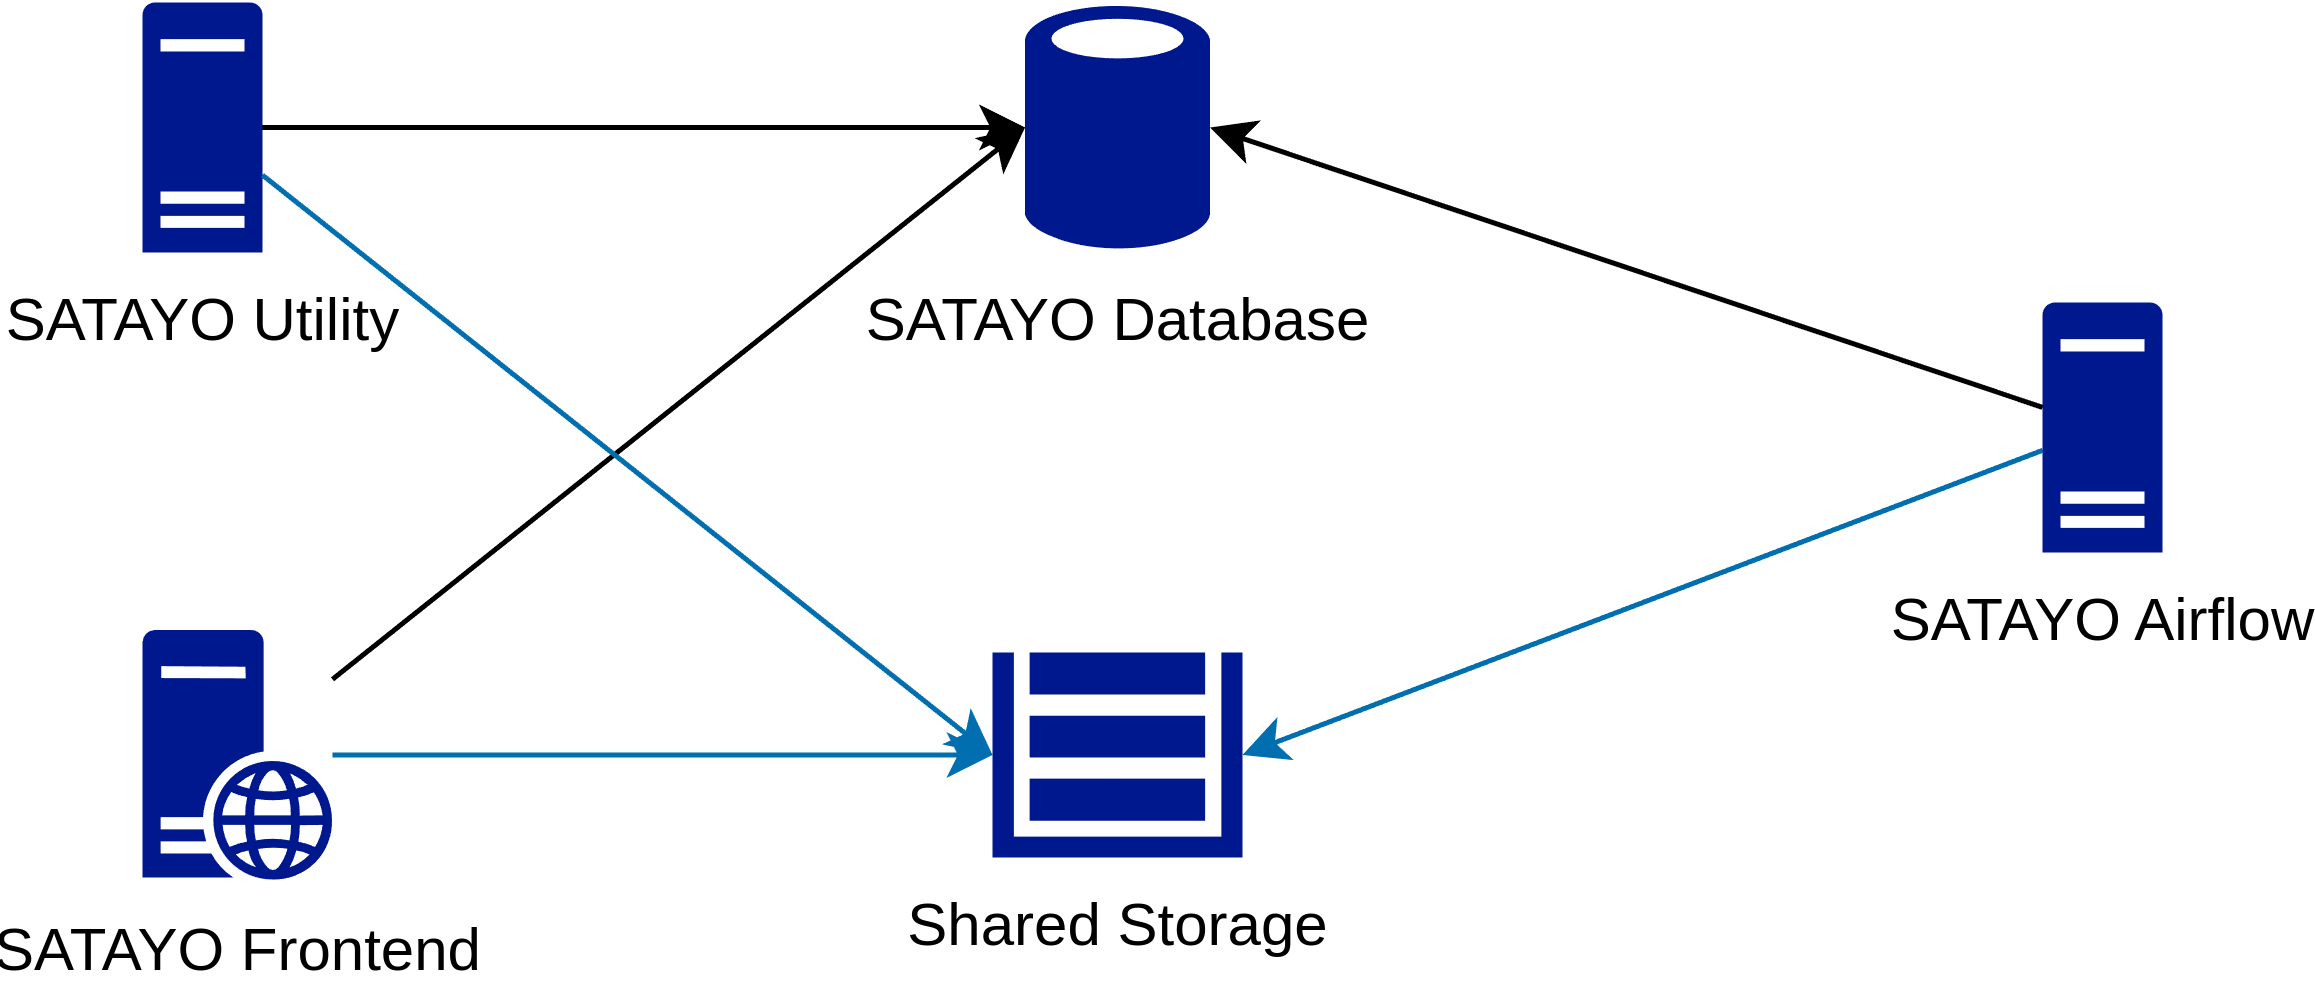
\includegraphics[width=.6\linewidth]{images/SATAYO_infrastructure_new.png}
  \caption{Nuova infrastruttura di SATAYO}
  \label{fig:infra_new}
\end{figure}

\section{Implementazione e Containerizzazione}
\label{sec:impl_container}

Dopo una prima analisi dei metodi di deployment messi a disposizione da Airflow,
è stato deciso di procedere inizialmente con l'utilizzo di un'immagine Docker\cite{docker}
istanziata su più container gestiti tramite Docker Compose. Nonostante questo approccio
sia sconsigliato dalla documentazione, che incita ad usare Kubernetes per gli
ambienti di produzione, è stato il modo più veloce per ottenere un'ambiente funzionante.
Sebbene possa sembrare, in primo luogo, che questa decisione porti ad un
ulteriore debito tecnico, non è assolutamente il caso. Il \texttt{Dockerfile} che
è stato scritto per questa implementazione, infatti, può essere utilizzato anche
per il deployment su Kubernetes.

Il \texttt{Dockerfile} descrivente l'immagine utilizzata, è stato implementato utilizzando
come base l'immagine ufficiale di Airflow \texttt{apache/airflow} e aggiungendo
tutte le dipendenze e tool OSINT utilizzati dalle fasi di SATAYO. Questo ha permesso
di semplificare l'implementazione delle fasi, in quanto non deve più essere
eseguito un controllo a tempo di esecuzione per verificare la presenza del tool
da eseguire. Le altre modifiche effettuate sul codice della vecchia implementazione
delle task, consultabile in \ref{lst:task-impl-old}, sono state: rimuovere il
controllo sul \texttt{id\_tool\_progress}, in quanto su Airflow l'esecuzione
della task avviene soltanto dopo che le sue dipendenze sono state risolte, non necessitando
quindi di controlli secondari all'interno della funzione stessa; aggiungere il
decoratore \texttt{@satayo\_task} all'inizio della definizione di ogni fase, il
quale ha la funzione di provvedere gli argomenti in modo tale che la nuova
implementazione sia compatibile con quella vecchia. Queste modifiche si possono osservare
nel codice nuovo \ref{lst:task-impl-new}, in cui viene direttamente eseguito il
corpo della fase.

Come precedentemente riportato, attualmente Airflow è utilizzato tramite Docker Compose,
è quindi in funzione su una macchina singola e l'infrastruttura è come riportato
in figura \ref{fig:infra_new}.

\pagebreak
\lstinputlisting[language=Python, caption=Esempio della precedente implementazione
di una fase di SATAYO, label=lst:task-impl-old]{listings/task-old.py}

\lstinputlisting[language=Python, caption=Esempio della nuova implementazione della
medesima fase, label=lst:task-impl-new]{listings/task-new.py}

\section{Retrocompatibilità}
\label{sec:retrocompatibility}

Per permettere una corretta integrazione del nuovo sistema all'interno di quello
corrente, mantenendo tutte le funzionalità presenti, è necessario continuare ad utilizzare
alcune funzionalità che potrebbero essere deprecate e sostituite interamente da Airflow.
In particolare occorre mantenere l'uso del \texttt{tool\_progress}, descritto
nella sezione \ref{sub:db:tasks}, in quanto questo viene utilizzato per calcolare
la data di ultima esecuzione di una determinata fase di SATAYO e per individuare
la fase che ha recuperato una certa evidenza. Per evitare la duplicazione di
codice è stato deciso di implementare questa funzionalità all'interno del
decoratore \texttt{@satayo\_task} (scritto utilizzando una classe Python) tramite
le due funzioni \texttt{pre\_task} e \texttt{post\_task}. L'implementazione
dettagliata è riportata in \ref{lst:retro}, si può notare come, nella prima
funzione, eseguita prima dell'esecuzione della task, venga utilizzato un \texttt{host\_id}
dedicato per le esecuzioni su Airflow, e sia creato un \texttt{tool\_progress} che
riporta le informazioni dell'esecuzione delle task come se venissero eseguite sul
sistema precedente. Nella seconda funzione, eseguita successivamente alla task,
viene invece impostata la data e lo stato di termine di essa. Per il caso di errore
di esecuzione viene chiamata una funzione di callback, presente tra gli
argomenti della task Airflow, che imposta il \texttt{tool\_progress} in stato di
errore.

Un'altra funzionalità riportata momentaneamente è la possibilità di salvare
certi messaggi di log all'interno del database. Questo è stato fatto per avere visibilità
su certi errori che non terminerebbero con errore la task, ma sarebbe comunque
opportuno controllare in caso si presentassero.

Infine è risultato necessario implementare anche un modo per delegare l'esecuzione
di alcune fasi al sistema vecchio, in quanto necessitanti di prerequisiti infrastrutturali
quali VPN o Proxy al momento non implementati all'interno del sistema basato su Airflow.
Ciò è stato ottenuto dividendo l'esecuzione in due parti: la prima task svolge la
funzionalità di creare un \textit{tool\_progress} e assegnarlo ad una macchina
Robot, la seconda è un \textit{Sensor} di Airflow che controlla con intervalli
regolari se la fase in questione è terminata e continua l'esecuzione del DAG in
base al risultato (successo continua l'esecuzione, errore viene interrotta e
notificata sulle dashboard descritte al punto \ref{sec:monitoraggio}).

\lstinputlisting[language=Python, caption={Implementazione delle funzioni di \texttt{@satayo\_task} che permettono la retrocompatibilità},
label=lst:retro]{listings/retrocompatibility-funcs.py}

\section{Ricerche schedulate}
\label{sec:schedulate}

\lstinputlisting[language=Python, caption={Funzione che calcola una schedulazione pseudo randomica per ogni dominio},
label=lst:schedule]{listings/schedule-generation.py}

Una delle funzionalità più interessanti di SATAYO per un cliente, è il monitoraggio
continuo della propria esposizione online. Per ottenere questo risultato è
essenziale eseguire determinate fasi secondo una schedulazione predefinita; nel dettaglio,
ci saranno delle task che devono essere eseguite giornalmente, settimanalmente o
ogni due settimane. Ciò è implementato dalle seguenti operazioni: viene eseguita
una query per collezionare la lista di domini da monitorare; da questa lista
vengono generati dinamicamente 3 DAG per ogni dominio, ognuno di essi contenente
le task da eseguire rispettivamente ogni giorno, settimana o due settimane. Per distribuire
equamente nel tempo le esecuzioni dei DAG settimanali e bisettimanali viene utilizzata
la funzione riportata in \ref{lst:schedule}. Il funzionamento di quest'ultima si
basa sul fatto che un PRNG (PseudoRandom Number Generator)\cite{py-random},
inizializzato con lo stesso \texttt{seed}, produrrà la medesima sequenza di
numeri. Utilizzando quindi come \texttt{seed} il dominio da analizzare, i DAG riferiti
ad esso verranno eseguiti con intervalli regolari e in giorni costanti. Per i
DAG settimanali verrà scelto un giorno casuale della settimana, mentre per quelli
bisettimanali verranno casualmente scelti due giorni del mese distanti 14 giorni.

\section{Nuove ricerche}
\label{sec:nuove}

\begin{figure}[htbp]
  \centering
  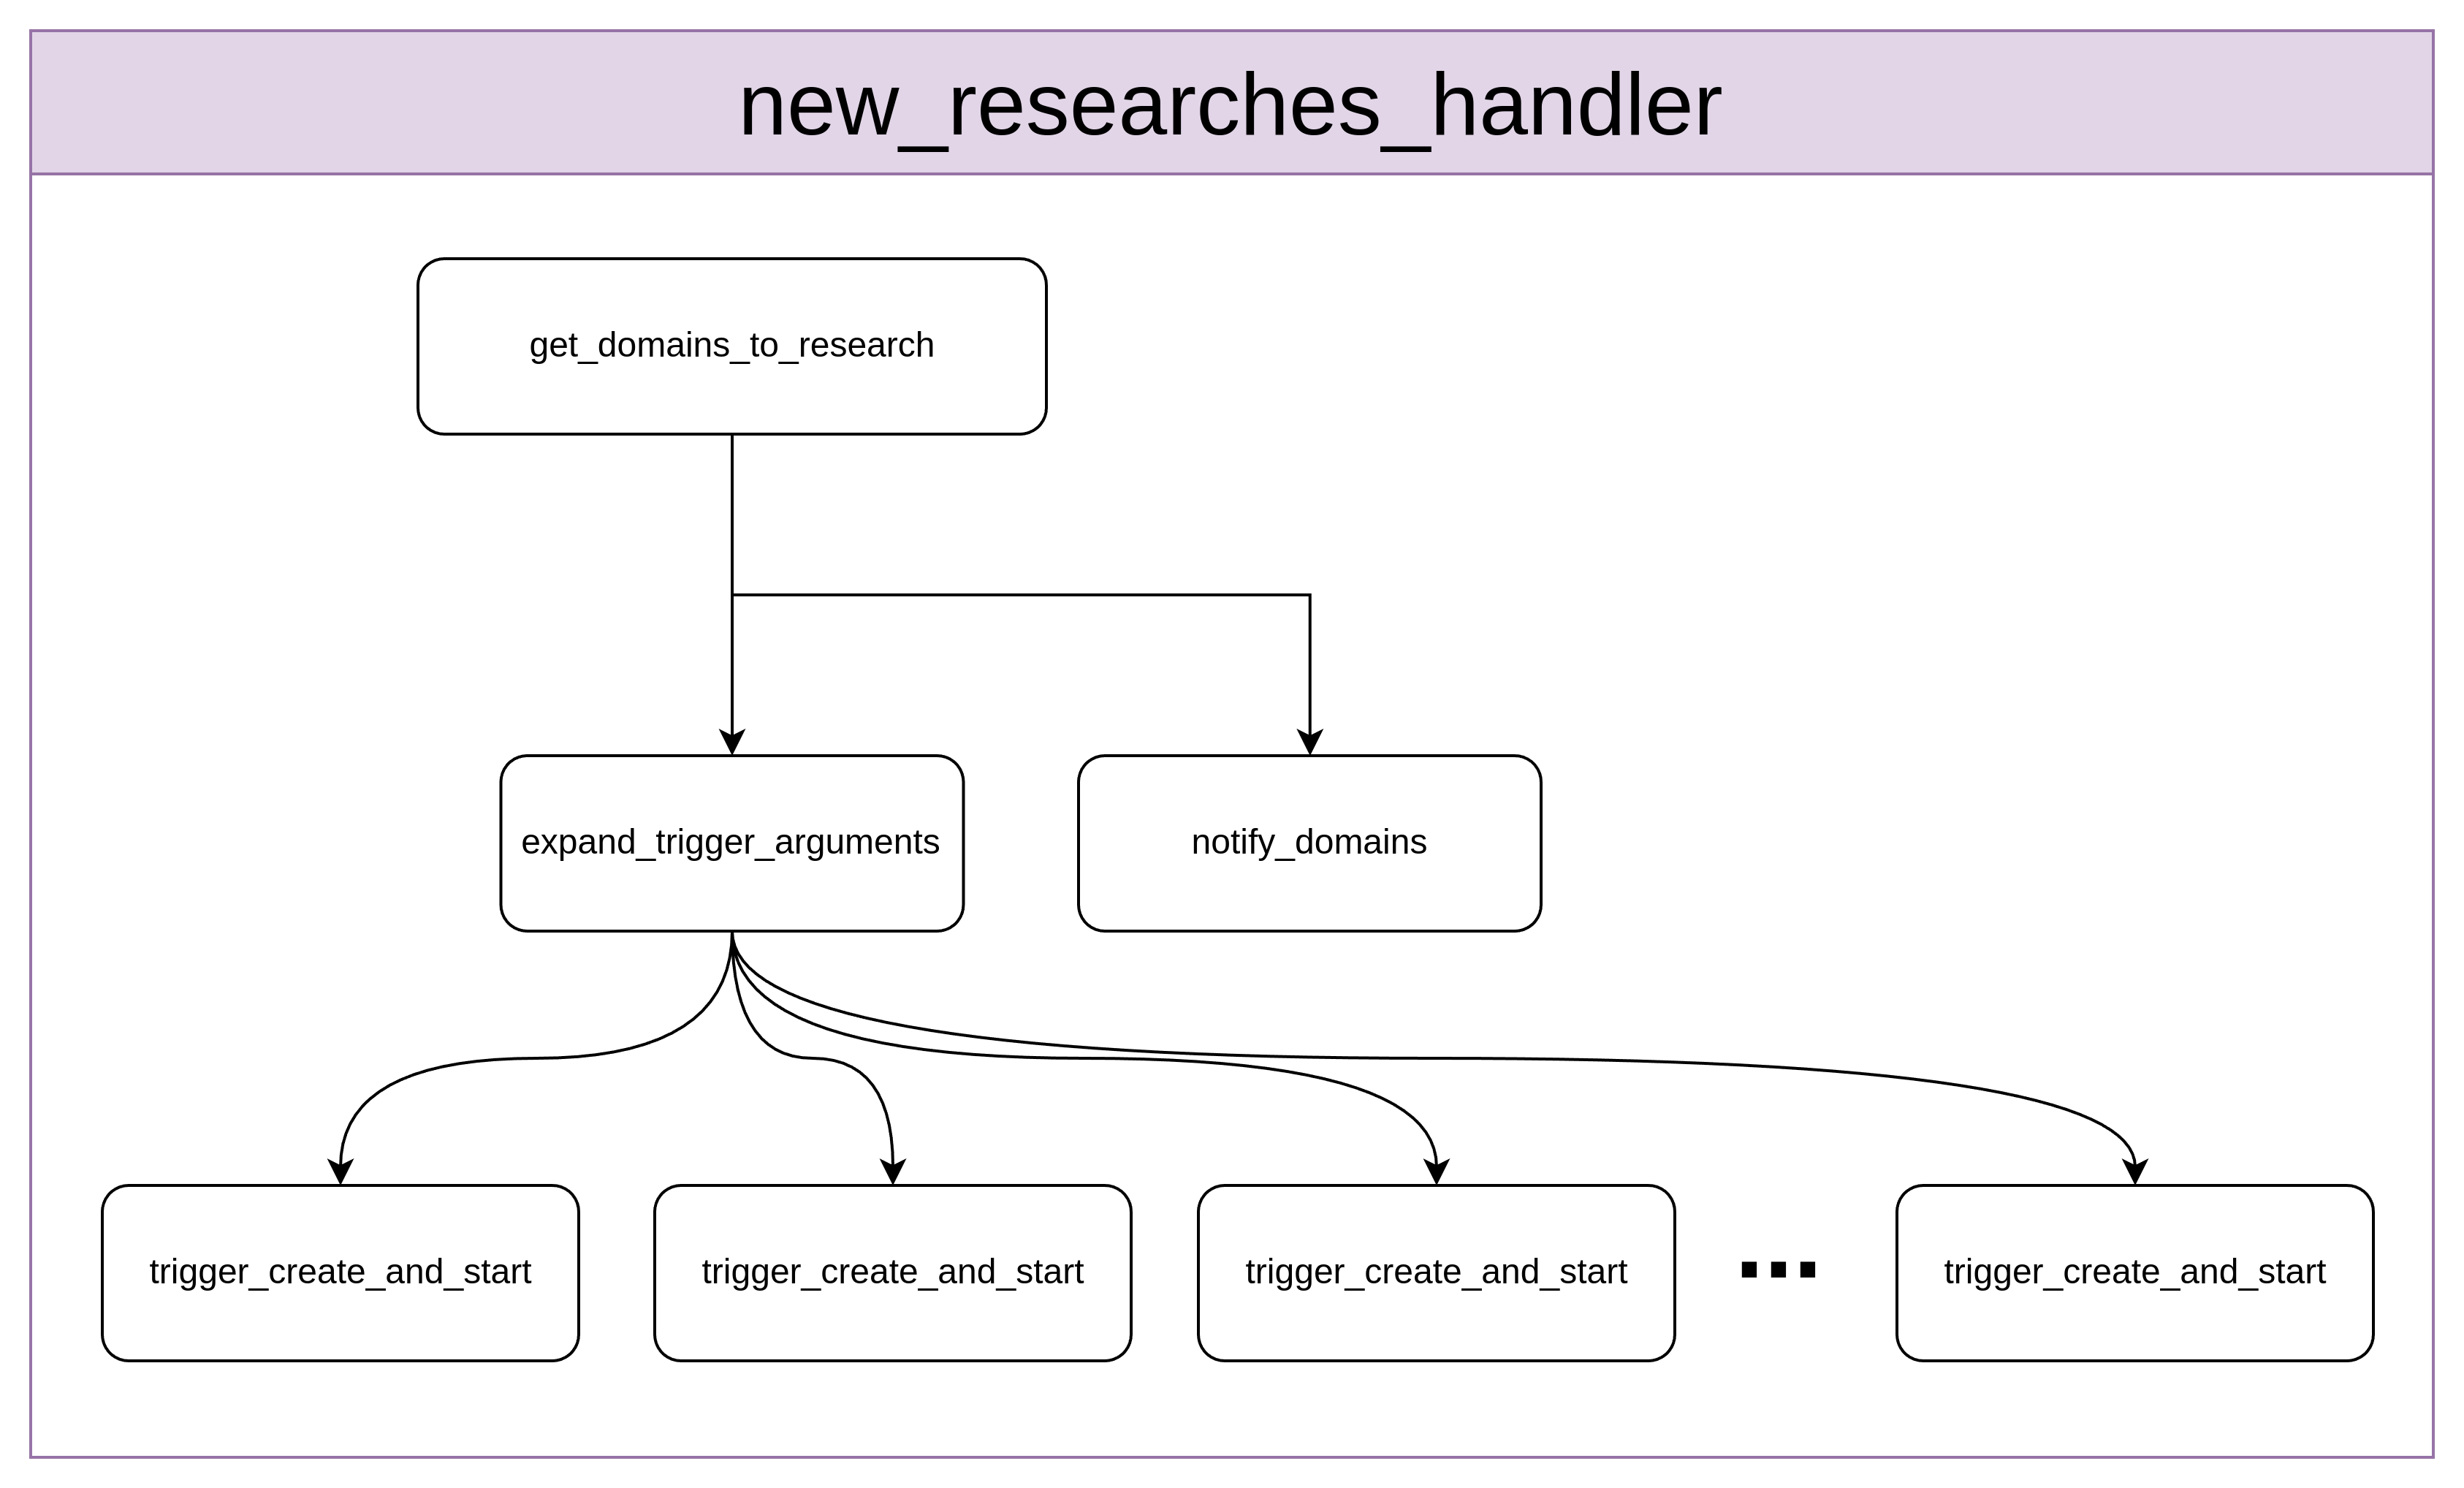
\includegraphics[width=.6\linewidth]{images/new_research_handler.png}
  \caption{DAG per gestire la schedulazione automatica di nuove ricerche}
  \label{fig:new-hanlder}
\end{figure}

Sebbene ci sia un monitoraggio continuo degli asset principali e più pericolosi,
in quanto più probabilmente utilizzati per organizzare campagne di Phishing, le fasi
ricorrenti non coprono tutto il perimetro dei clienti. Per questo è necessario
eseguire in modo ricorrente anche i controlli più pesanti e lunghi, ovviamente con
minore frequenza. Dato il più alto carico computazionale, è stato scelto di utilizzare
un approccio più controllato per schedulare i DAG delle nuove ricerche \texttt{start\_new\_research}.
Nel dettaglio è presente un DAG \texttt{new\_research\_handler} che ha il
compito di: collezionare i domini di cui eseguire la nuova ricerca, notificare
tali domini prima dell'inizio dell'esecuzione delle ricerche e creare ed avviare
le nuove ricerche stesse. Questo DAG viene eseguito tre volte al giorno in orario
lavorativo, in quanto i DAG ricorrenti vengono eseguiti di notte, in modo tale di
poter intervenire in caso di malfunzionamenti. Analizzando il DAG riportato in
figura \ref{fig:new-hanlder}, si può notare la presenza delle seguenti task:

\begin{itemize}
  \item \textbf{get\_domains\_to\_research:} la quale raccoglie in base all'età
    della ricerca e ad altri parametri i domini per cui creare una nuova ricerca.
    Colleziona inoltre anche i domini di cui è stata richiesta manualmente l'esecuzione
    di una ricerca completa. Questa task genera una lista di domini che verrà
    passata alla task successiva;

  \item \textbf{notify\_domains:} implementa un sistema di notifica tramite
    messaggio di notifica con Bot Telegram\footnote{\url{https://core.telegram.org/bots}},
    questo permette di avere una visione immediata e di alto livello sulle nuove
    ricerche che stanno per essere eseguite. Questo è importante perché, come
    specificato precedentemente, si tratta di un'operazione importante che, in
    caso di malfunzionamenti potrebbe portare a gravi ripercussioni;

  \item \textbf{expand\_trigger\_arguments:} è una task di natura puramente
    implementativa, serve cioè soltanto a convertire la lista di domini fornita da
    \texttt{get\_domains\_to\_research} in un formato tale da essere compatibile
    con le task successive. Viene quindi, per ogni dominio, creato un \texttt{trigger\_run\_id}
    e un oggetto \texttt{conf} che verranno passati alla task successiva, la
    quale avrà effettivamente il compito di avviare le nuove ricerche;

  \item \textbf{trigger\_create\_and\_start:} ha il compito fondamentale di
    eseguire il DAG responsabile della creazione della nuova ricerca sul
    database, \texttt{create\_and\_start\_new\_research}, la quale viene eseguita
    importando tutte le informazioni utili dalla ricerca precedente, e dell'avvio
    vero e proprio del DAG \texttt{start\_new\_research} incaricato di eseguire effettivamente
    tutte le task necessarie a svolgere una nuova ricerca. Questa task viene
    generata in modo dinamico in base agli oggetti presenti nella lista generata
    allo step precedente che corrispondono al numero di domini per cui
    istanziare una nuova ricerca. In seguito, ciascuna Task Instance creerà una
    DAG Run differente, del medesimo DAG, per ogni oggetto nella lista.
\end{itemize}

\section{Task di sistema}
\label{sec:sistema}

Per una corretta integrazione con il vecchio sistema di SATAYO è stato necessario
creare delle routine di sincronizzazione. In particolare viene riportata una
descrizione della task \texttt{satayo\_tp\_sync}, responsabile della
sincronizzazione dello stato dei tool\_progress sul database di SATAYO con lo
stato effettivo presente su Airflow. La task in questione è necessaria in quanto
possono verificarsi dei casi in cui le funzioni \texttt{pre\_task} e \texttt{post\_task}
descritte al punto \ref{sec:retrocompatibility} non vengano eseguite correttamente.
I casi in questione sono principalmente interventi manuali sullo stato delle
task. Per evitare l'inserimento di logiche inutilmente complesse all'interno della
definizione delle task è stata implementata una task dedicata, eseguita ogni 10
minuti, che gestisce i seguenti due casi:

\begin{itemize}
  \item se viene trovato un tool\_progress che individua la task come in esecuzione
    e, al contrario, all'interno di Airflow tale task non ha lo stato \textit{running},
    essa viene impostata, all'interno del db di SATAYO come \textit{failed};

  \item al contrario invece, se all'interno della tabella dei tool\_progress
    viene trovata una fase in stato \textit{failed}, ma all'interno di Airflow
    essa è riportata con lo stato \textit{success}, ne viene cambiato lo stato
    sul database e impostato anch'esso a \textit{success}. Questo comportamento
    capita spesso nel caso in cui una task, terminata in errore, venga eseguita
    un secondo momento, creando un ulteriore tool\_progress.
\end{itemize}

A seguito di entrambe le precedenti azioni, vengono inoltre inseriti dei messaggi
di log all'interno della tabella \texttt{log} del database di SATAYO, per permettere
una migliore visibilità delle azioni della routine.

\section{Testing e rilascio in produzione}
\label{sec:deployment}

Avendo a disposizione un ambiente di test limitato è stato deciso di utilizzare
la strategia di rilascio \textit{Canary Deployment Strategy}\cite{humble2010continuous}.
Il motivo principale della presenza di un contesto di test particolarmente ridotto
è la natura del progetto. Molte funzionalità di SATAYO infatti si basano sul
fatto di avere a disposizione lo storico delle informazioni collezionate sui
domini in analisi. Questo può essere simulato in un ambiente di test, ma non è
possibile riportare le informazioni come se fosse un environment di produzione
vero e proprio. Un secondo problema, dettato dalla complessità del progetto, è la
quantità ingente di fasi, ricorrenti e non, eseguite in produzione. Questo non
permette infatti di utilizzare ambienti di test per fare prove di carico senza
utilizzare un'infrastruttura identica a quella di produzione.

Per validare quindi i risultati ottenuti dalla nuova implementazione è stata
utilizzata la strategia \textit{A/B Testing}\cite{QUIN2024112011}, che consiste nell'eseguire
la stessa operazione su due versioni diverse della stessa applicazione e confrontare
i risultati. In questo caso sono state eseguite delle ricerche complete sullo
stesso dominio, su entrambe le infrastrutture e sono stati paragonati, alla
vecchia implementazione, il numero e la qualità dei risultati ottenuti dalla nuova.

Infine è stata eseguita la procedura di \textit{Canary Deployment} menzionata
prima per migrare la vecchia versione a quella nuova. Il \textit{Canary
Deployment} consiste nel migrare gradualmente il carico di lavoro da una istanza
ad un'altra, avente una versione più recente del software. Nel caso specifico di
SATAYO sono state inizialmente migrate le fasi ricorrenti, procedendo con batch di
circa 100 domini alla settimana. Una volta terminata la migrazione delle fasi
schedulate, si è passati alla migrazione delle nuove ricerche, che inizialmente
venivano eseguite manualmente sulla nuova piattaforma, ed in seguito, a
migrazione completa, sono state automatizzate.

\section{Monitoraggio}
\label{sec:monitoraggio}

Ultimo sviluppo fondamentale per ottenere un sistema pronto al rilascio in
produzione è stata l'implementazione di un sistema di monitoraggio. I requisiti di
un tale sistema sono: una visione di insieme dello stato di esecuzione dei DAG e
altre interfacce che presentino informazioni relative a tutto il sistema con
maggiori dettagli e granularità. Per l'implementazione delle dashboard in questione
è stato utilizzato il modulo di NetEye \textit{ITOA} (IT Operations Analytics), il
quale è realizzato utilizzando il software di visualizzazione Open source \textbf{Grafana}\footnote{\url{https://grafana.com/grafana/}}.
Nello specifico è stata realizzata una dashboard che include tutte le
informazioni importanti riguardanti lo stato del sistema, la quale è presentata in
figura \ref{fig:main_dash}. In questa visualizzazione sono presenti informazioni
quali: il numero di fasi in errore, divise per tipologia (Airflow o Robot); il \textit{tempo
macchina} utilizzato, inteso come tempo utilizzato dall'esecuzione delle task considerato
sul numero massimo di task eseguibili in parallelo; le fasi in esecuzione e
altre informazioni riguardanti le code dei due sistemi. Una seconda dashboard di
rilievo è sicuramente la \textit{Airflow Failed Management}\ref{fig:errors_dash},
utilizzata appunto per gestire e rilanciare le fasi che hanno prodotto errori di
esecuzione. In questa dashboard è possibile notare una visualizzazione generale,
divisa per tipologia di DAG a cui appartengono le task in errore e un'aggregazione
del numero di fasi diverse che hanno prodotto errori. Al centro è presente una tabella
con tutti gli errori da gestire e link rapidi alle rispettive pagine di log.
Entrambe le dashboard hanno associato ad ogni pannello un link rapido alla
pagina inerente all'informazione mostrata. Oltre a queste sono presenti anche altre
visualizzazioni quali: un'aggregazione di statistiche di esecuzione delle fasi, monitoraggio
delle API utilizzate dai vari servizi a pagamento sui quali si basa SATAYO e storico
dell'utilizzo di \textit{tempo macchina}.

\begin{figure}[htbp]
  \centering
  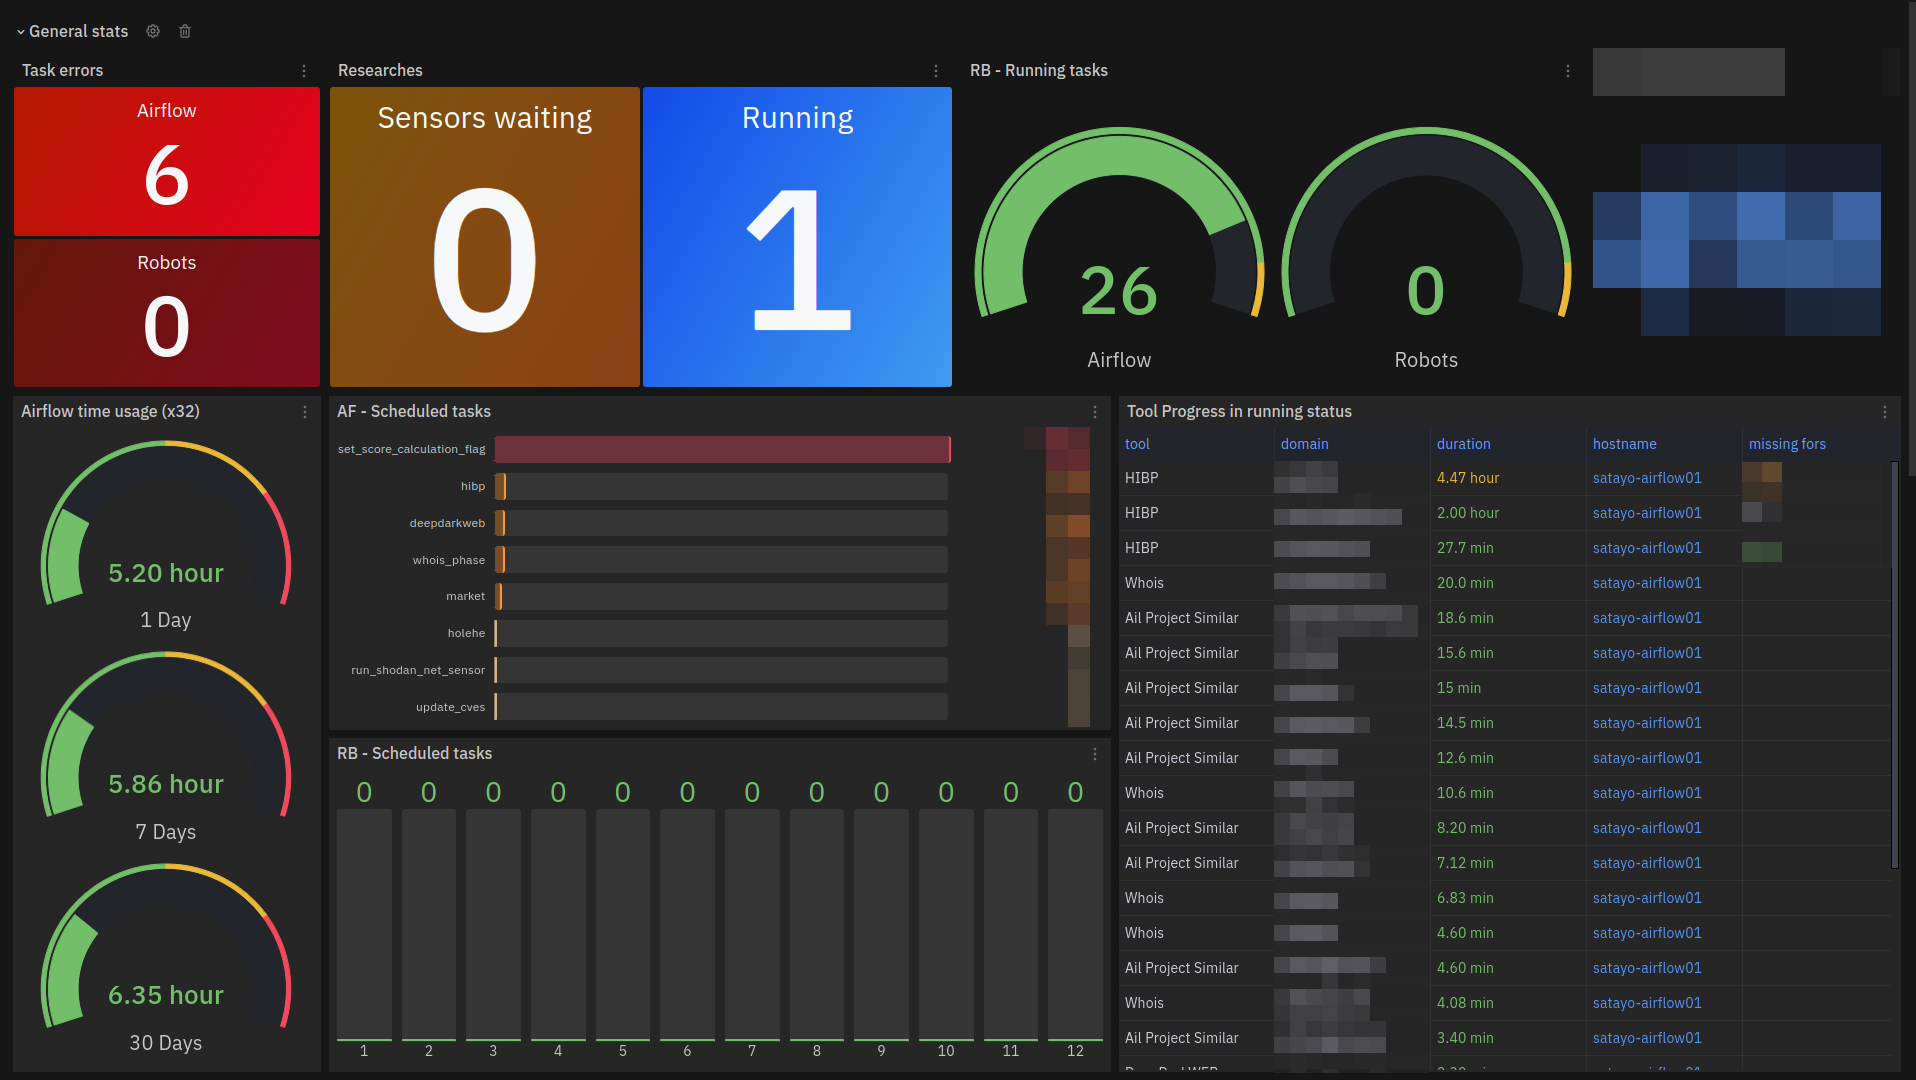
\includegraphics[width=.9\linewidth]{images/SATAYO_main_dashboard.png}
  \caption{Dashboard principale di SATAYO}
  \label{fig:main_dash}
\end{figure}

\begin{figure}[htbp]
  \centering
  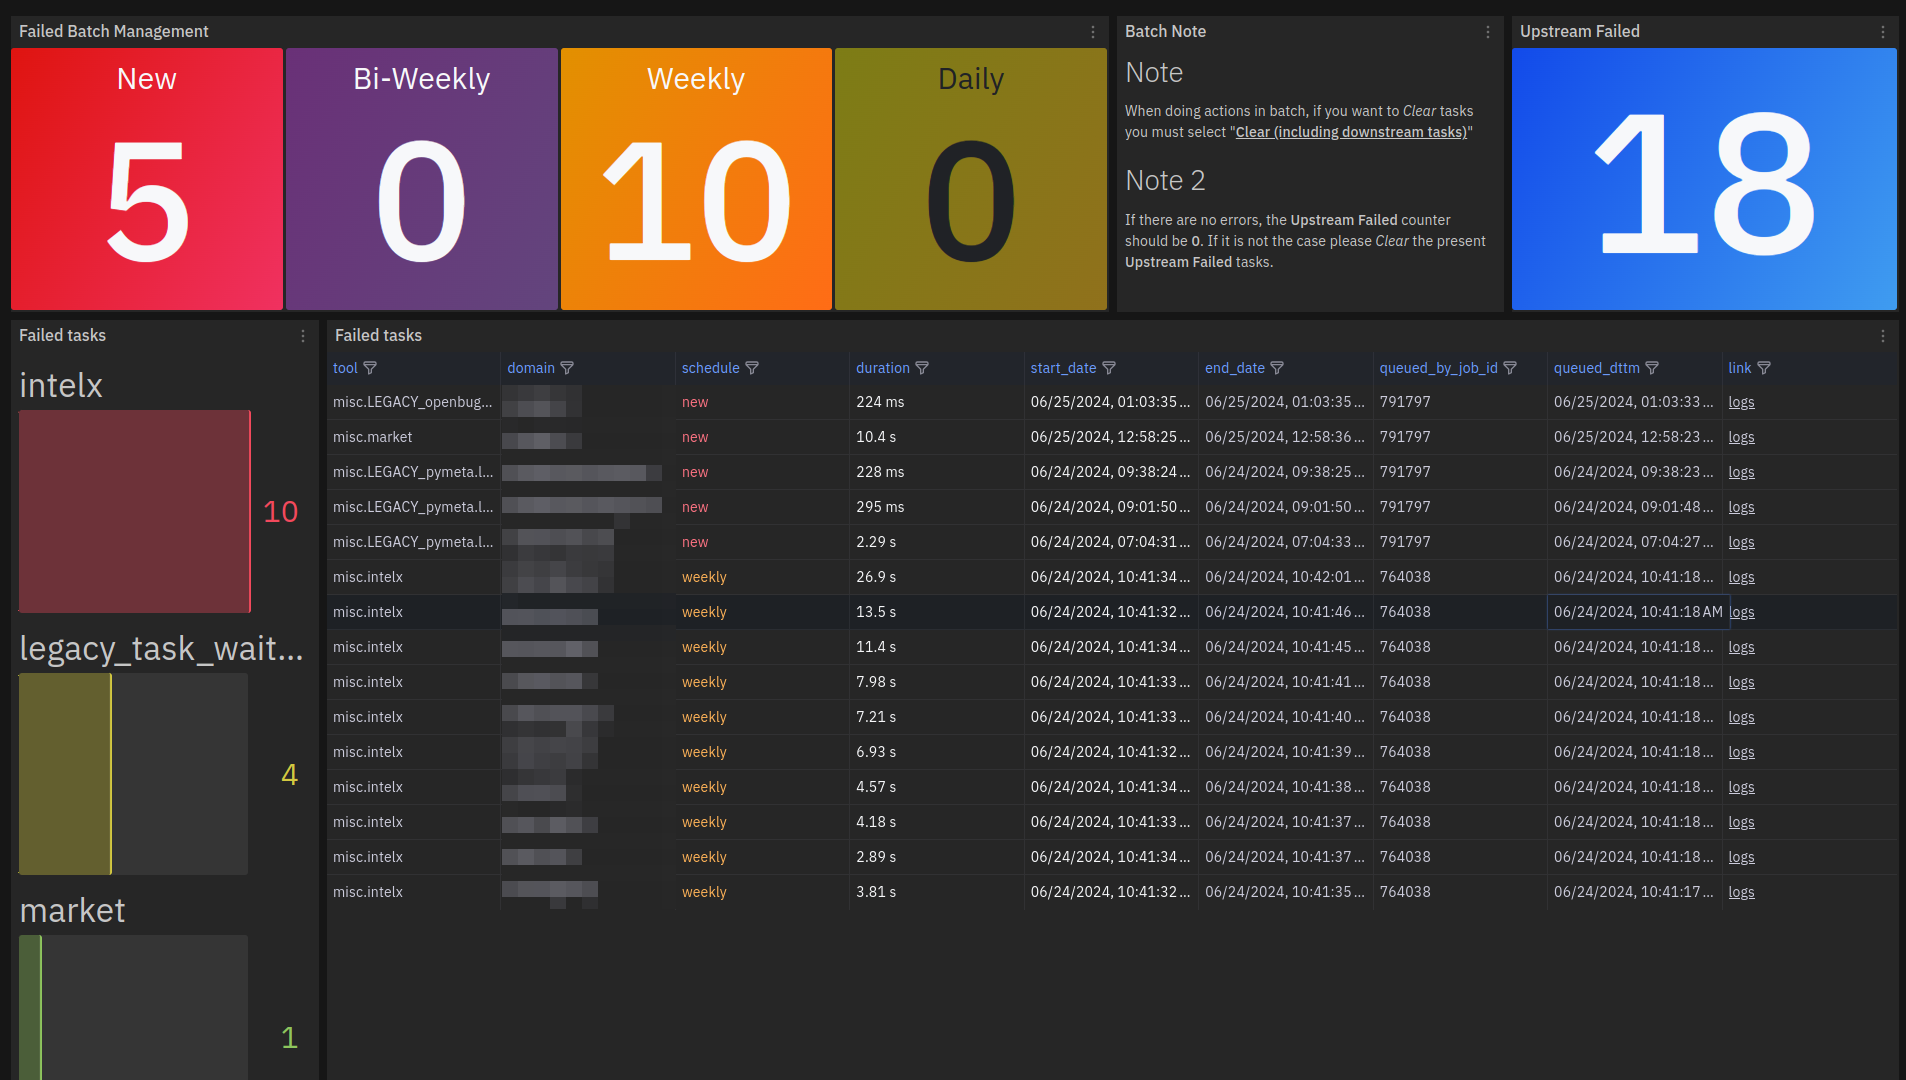
\includegraphics[width=.9\linewidth]{images/SATAYO_errors_dashboard.png}
  \caption{Dashboard di gestione errori di SATAYO}
  \label{fig:errors_dash}
\end{figure}

  % Conclusions
  \chapter{Conclusioni}
\label{cha:conclusioni}

Individuato il problema principale dell'implementazione precedente, con questi nuovi
sviluppi, il progetto SATAYO ha visto una rivisitazione completa del proprio
core. Per fare ciò sono state analizzate molte alternative all'architettura passata,
tra cui alla fine è stata scelta la più adeguata secondo i requisiti definiti
durante la fase di analisi. Questo ha portato a un netto miglioramento della capacità
di analisi del sistema e ad una riduzione di risorse utilizzate in totale.

Durante l'analisi dell'applicazione e il processo di implementazione e migrazione
al nuovo sistema, sono state inoltre individuate altre aree in cui si potrebbero
apportare ulteriori migliorie. Sono riportate di seguito le principali e di più rilievo:

\begin{itemize}
  \item \textbf{Implementazione con Kubernetes:} è il prossimo sviluppo che
    emerge scontato dalla nuova implementazione. Come accennato al punto \ref{sec:impl_container}
    la configurazione dei container attuale, basata su Docker Compose, non è consigliata
    per carichi di lavoro di produzione. Per questo motivo è presente il \texttt{Helm
    Chart}\footnote{\url{https://helm.sh/docs/topics/charts/}} ufficiale messo a
    disposizione dagli sviluppatori di Airflow, il quale descrive l'infrastruttura
    ideale da dispiegare all'interno del cluster Kubernetes, per ottenere un
    funzionamento ottimale del sistema. Il Helm Chart permette inoltre di utilizzare
    immagini Docker customizzate, permettendo quindi di usare direttamente l'immagine
    sviluppata per l'implementazione attuale. Questa miglioria, illustrata nell'immagine
    \ref{fig:infra_future}, porterà ad avere maggiore capacità di calcolo ed affidabilità
    all'interno di Airflow, permettendo quindi lo sviluppo riportato al prossimo
    punto;

  \item \textbf{Migrazione fasi Utility:} in ottica di manutenibilità del
    progetto e di standardizzazione dello stile del codice e delle regole di
    formattazione e linting, sarebbe opportuno migrare anche le fasi Utility al sistema
    Airflow. Dato il fatto che queste fasi hanno requisiti di isolamento
    particolari, per eseguire la migrazione è necessario testare a fondo il DockerOperator,
    introdotto nella sezione \ref{sec:airflow}, in modo tale da assicurarsi il corretto
    funzionamento delle fasi menzionate all'interrno del nuovo ambiente;

  \item \textbf{Aggregazione e analisi dei log:} altra funzionalità utile dal
    punto di vista del monitoraggio dell'esecuzione delle task è sicuramente il
    collezionamento e l'aggregazione dei log. Sarebbe ideale utilizzare direttamente
    il servizio messo a disposizione da NetEye, che permetterebbe di indicizzare
    i messaggi di log completi prodotti dalle task di Airflow su Elasticsearch. In
    questo modo sarebbe possibile, oltre a consultare dettagliatamente i
    messaggi di log prodotti, anche creare una dashboard su Kibana\footnote{\url{https://www.elastic.co/kibana}}.
    Tale dashboard permetterebbe di avere visibilità su determinate tipologie di
    errore non critico che altrimenti verrebbe ignorato, rendendo possibile l'individuazione
    di bug che potrebbero portare alla perdita di informazione;

  \item \textbf{Pipeline di CI/CD e test automatizzati:} attualmente, la procedura
    di aggiornamento della versione di SATAYO Airflow viene effettuata manualmente.
    Sulla macchina di produzione vengono svolte le seguenti azioni: viene aggiornato
    il codice presente in locale, eseguita la procedura di build dell'immagine
    Docker, e infine vengono avviati i nuovi container basati sulla nuova versione.
    Tutte queste procedure potrebbero essere automatizzate tramite una pipeline
    di Continuous Deployment, responsabile di: costruire l'immagine del
    Container, e scaricarla ed avviarla automaticamente sull'istanza di produzione.
    Avere a disposizione l'immagine permetterebbe anche l'esecuzione di test
    automatizzati in un ambiente analogo a quello effettivo, permettendo quindi di
    testare automaticamente l'intera applicazione;

  \item \textbf{Notifiche intelligenti:} ultima feature molto valida sarebbe
    appunto un sistema di notifiche immediate in caso di errori. Nello specifico
    verrebbe utilizzato un servizion di messaggistica istantanea, e.g. Telegram,
    per permettere la ricezione di notifiche in ogni momento. Gli eventi notificabili
    tramite questo sistema sarebbero principalmente errori critici di fasi di sistema
    e, secondariamente, errori di esecuzione delle task di SATAYO. Quest'ultima
    categoria di notifiche potrebbe portare in certi casi a spam indesiderato, per
    questo sarebbe opportuno attendere che le fasi di SATAYO raggiungano un'affidabilità
    tale da non risultare in troppe notifiche o, alternativamente, bisognerebbe implementare
    un rate limit per limitare le notifiche inviate.
\end{itemize}

\begin{figure}[htbp]
  \centering
  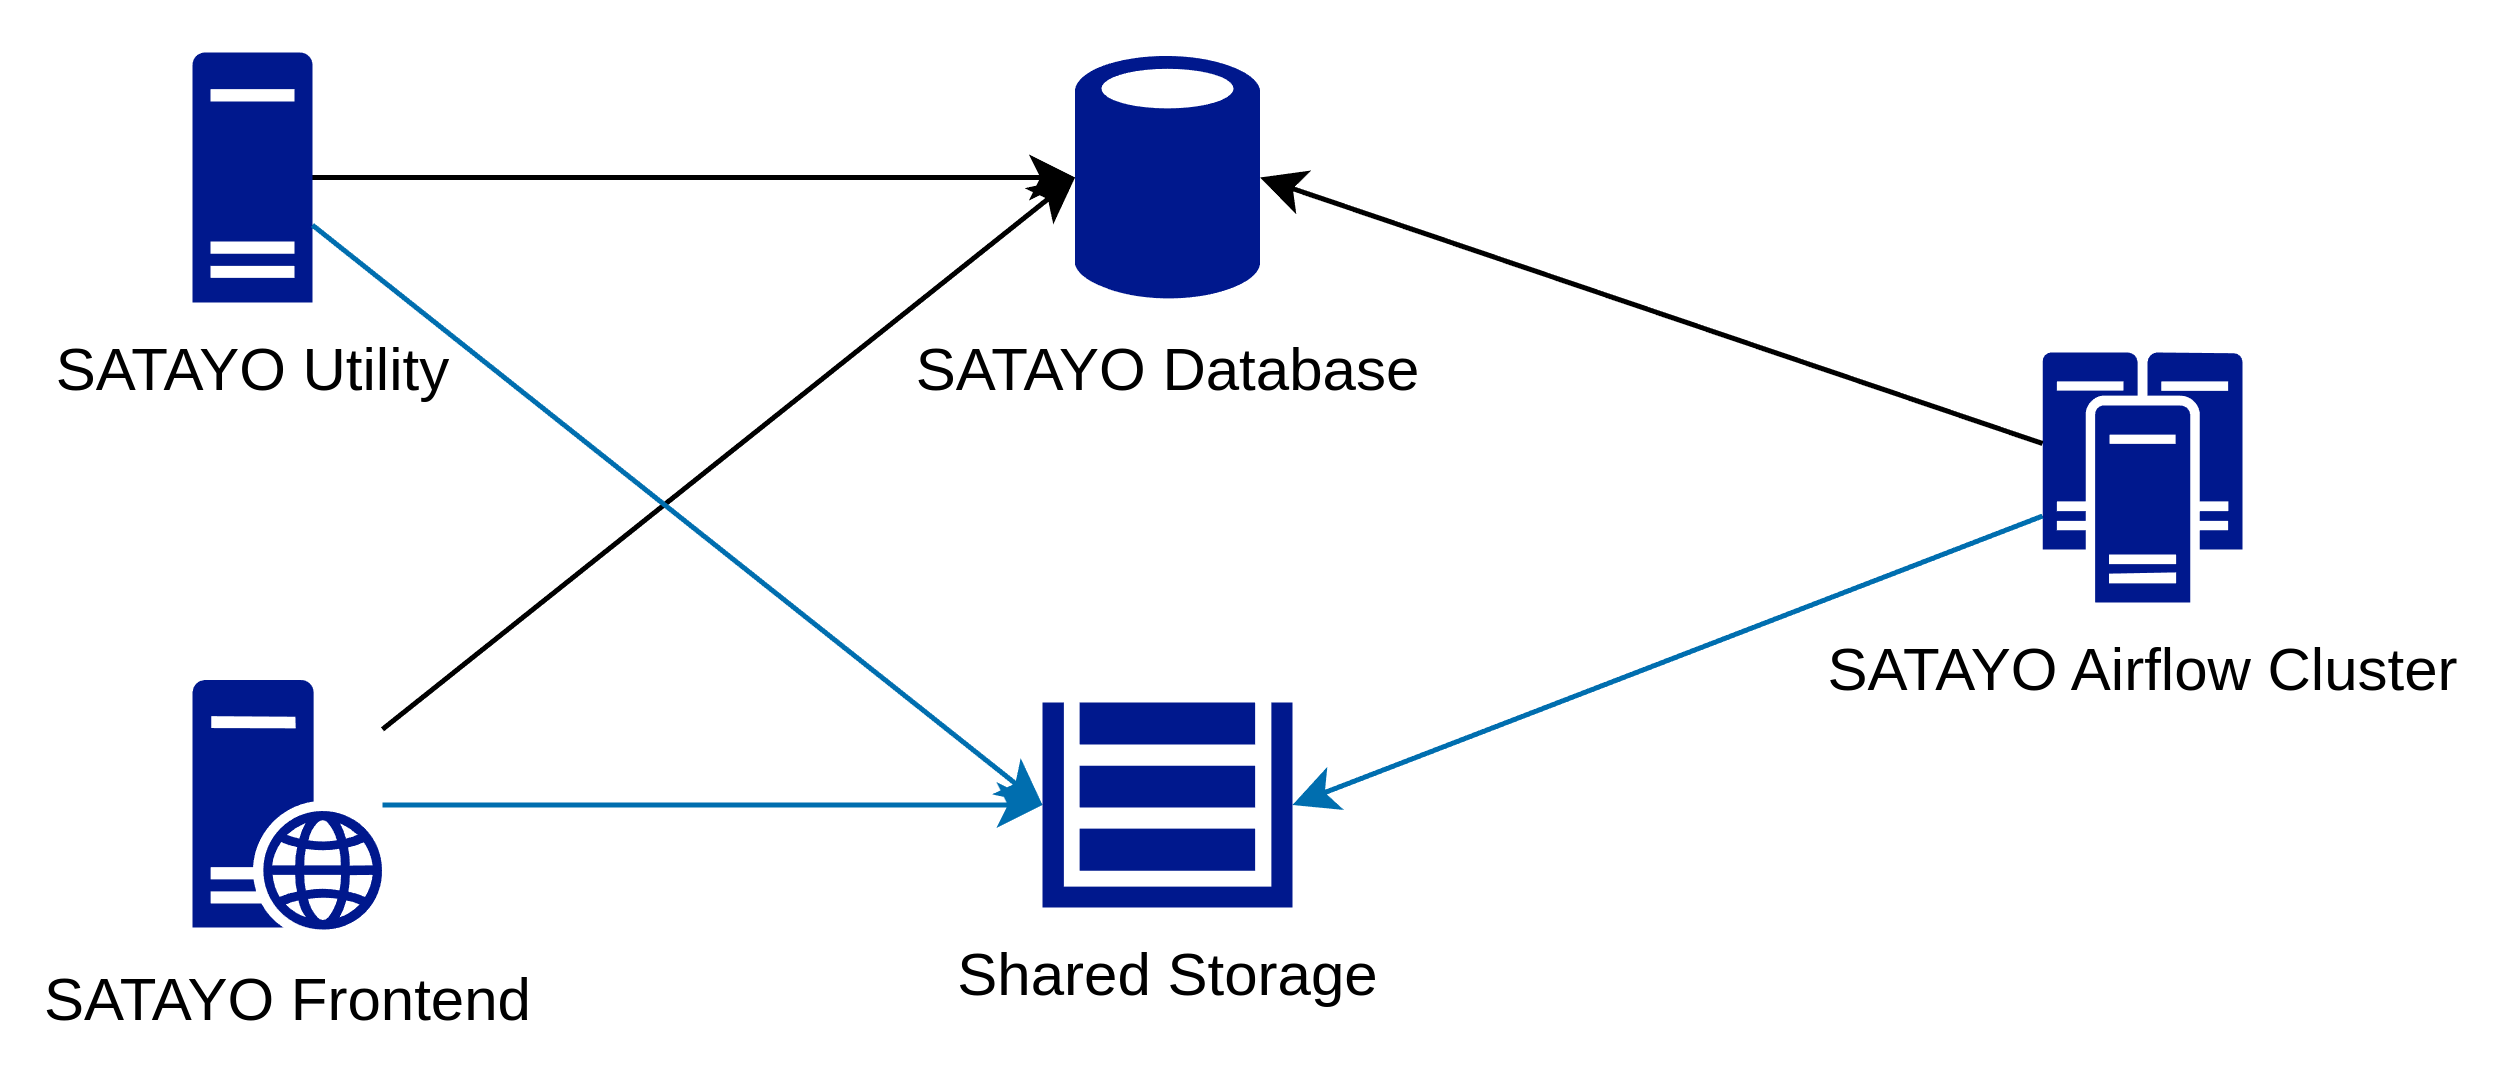
\includegraphics[width=.6\linewidth]{images/SATAYO_infrastructure_future.png}
  \caption{Futura infrastruttura di SATAYO}
  \label{fig:infra_future}
\end{figure}

  \endgroup

  % Bibliography
  \addcontentsline{toc}{chapter}{Bibliografia}
  % Alphabetical order of authors
  \bibliographystyle{plain}
  \bibliography{bibliography.bib}
\end{document}